\hypertarget{measurement-and-data-collection}{%
\section{Measurement and Data
Collection}\label{measurement-and-data-collection}}

This section enumerates the procedure for measuring AIT. Researchers
should follow these procedures every day and for every experiment
performed to ensure consistent results. The first priority should always
be safety. Therefore, if any step of this process is found to be unsafe
or pose an unacceptable risk it should be changed. This method is
designed to conform to the ASTM E659 Method. Therefore, any policies and
procedures violate standards set forth in ASTM E659 should be rectified
to maintain conformity.

\hypertarget{startup}{%
\subsection{Startup}\label{startup}}

\begin{enumerate}
\def\labelenumi{\arabic{enumi}.}
\item
  Ensure the lid is off the pressure vessel and the vessel is being
  vented by the snorkel

  \begin{itemize}
  \tightlist
  \item
    Under normal operation, the vessel should be vented with the snorkel
    any time the vessel is open
  \item
    The only exception to this rule is when the experimental setup has
    been shut down for an extended period of time for maintenance
    purposes
  \end{itemize}
\item
  Check the lab book to see if the flask needs to be changed before
  turning on the furnace. If needed, change the flask (See Section
  \ref{sec:flask-and-lid} ) and \textbf{indicate you did so in the lab
  notebook}.
\item
  Ensure the furnace is plugged in to the 220 V outlet on the edge of
  the hood
\item
  Power on the furnace and set furnace temperature between 10 - 20
  degrees above your initial target flask temperature

  \begin{itemize}
  \tightlist
  \item
    When powered on initially, the furnace may take 2 hours or more to
    reach a desired temperature and thermally equilibrate
  \item
    Use the TADA\_UI to track the internal temperature of the flask
  \item
    Once the internal temperature starts to reach equilibrium, you may
    adjust the set point temperature until the target temperature is
    reached
  \item
    \textbf{CAUTION: The furnace may be hot during the start up
    sequence. Avoid touching anything inside the area enclosed by the
    aluminum ring atop the furnace including the ring itself.}
  \end{itemize}
\item
  Ensure the vessel rupture disk is intact and positioned correctly (See
  Figure \ref{fig:rupture_disk})

  \begin{enumerate}
  \def\labelenumii{\arabic{enumii}.}
  \tightlist
  \item
    See the training on proper rupture disk installation (Section
    \ref{sec:Changing-the-rupture-disk}) if the this is not the case
  \end{enumerate}

  \begin{figure}
  \hypertarget{fig:rupture_disk}{%
  \centering
  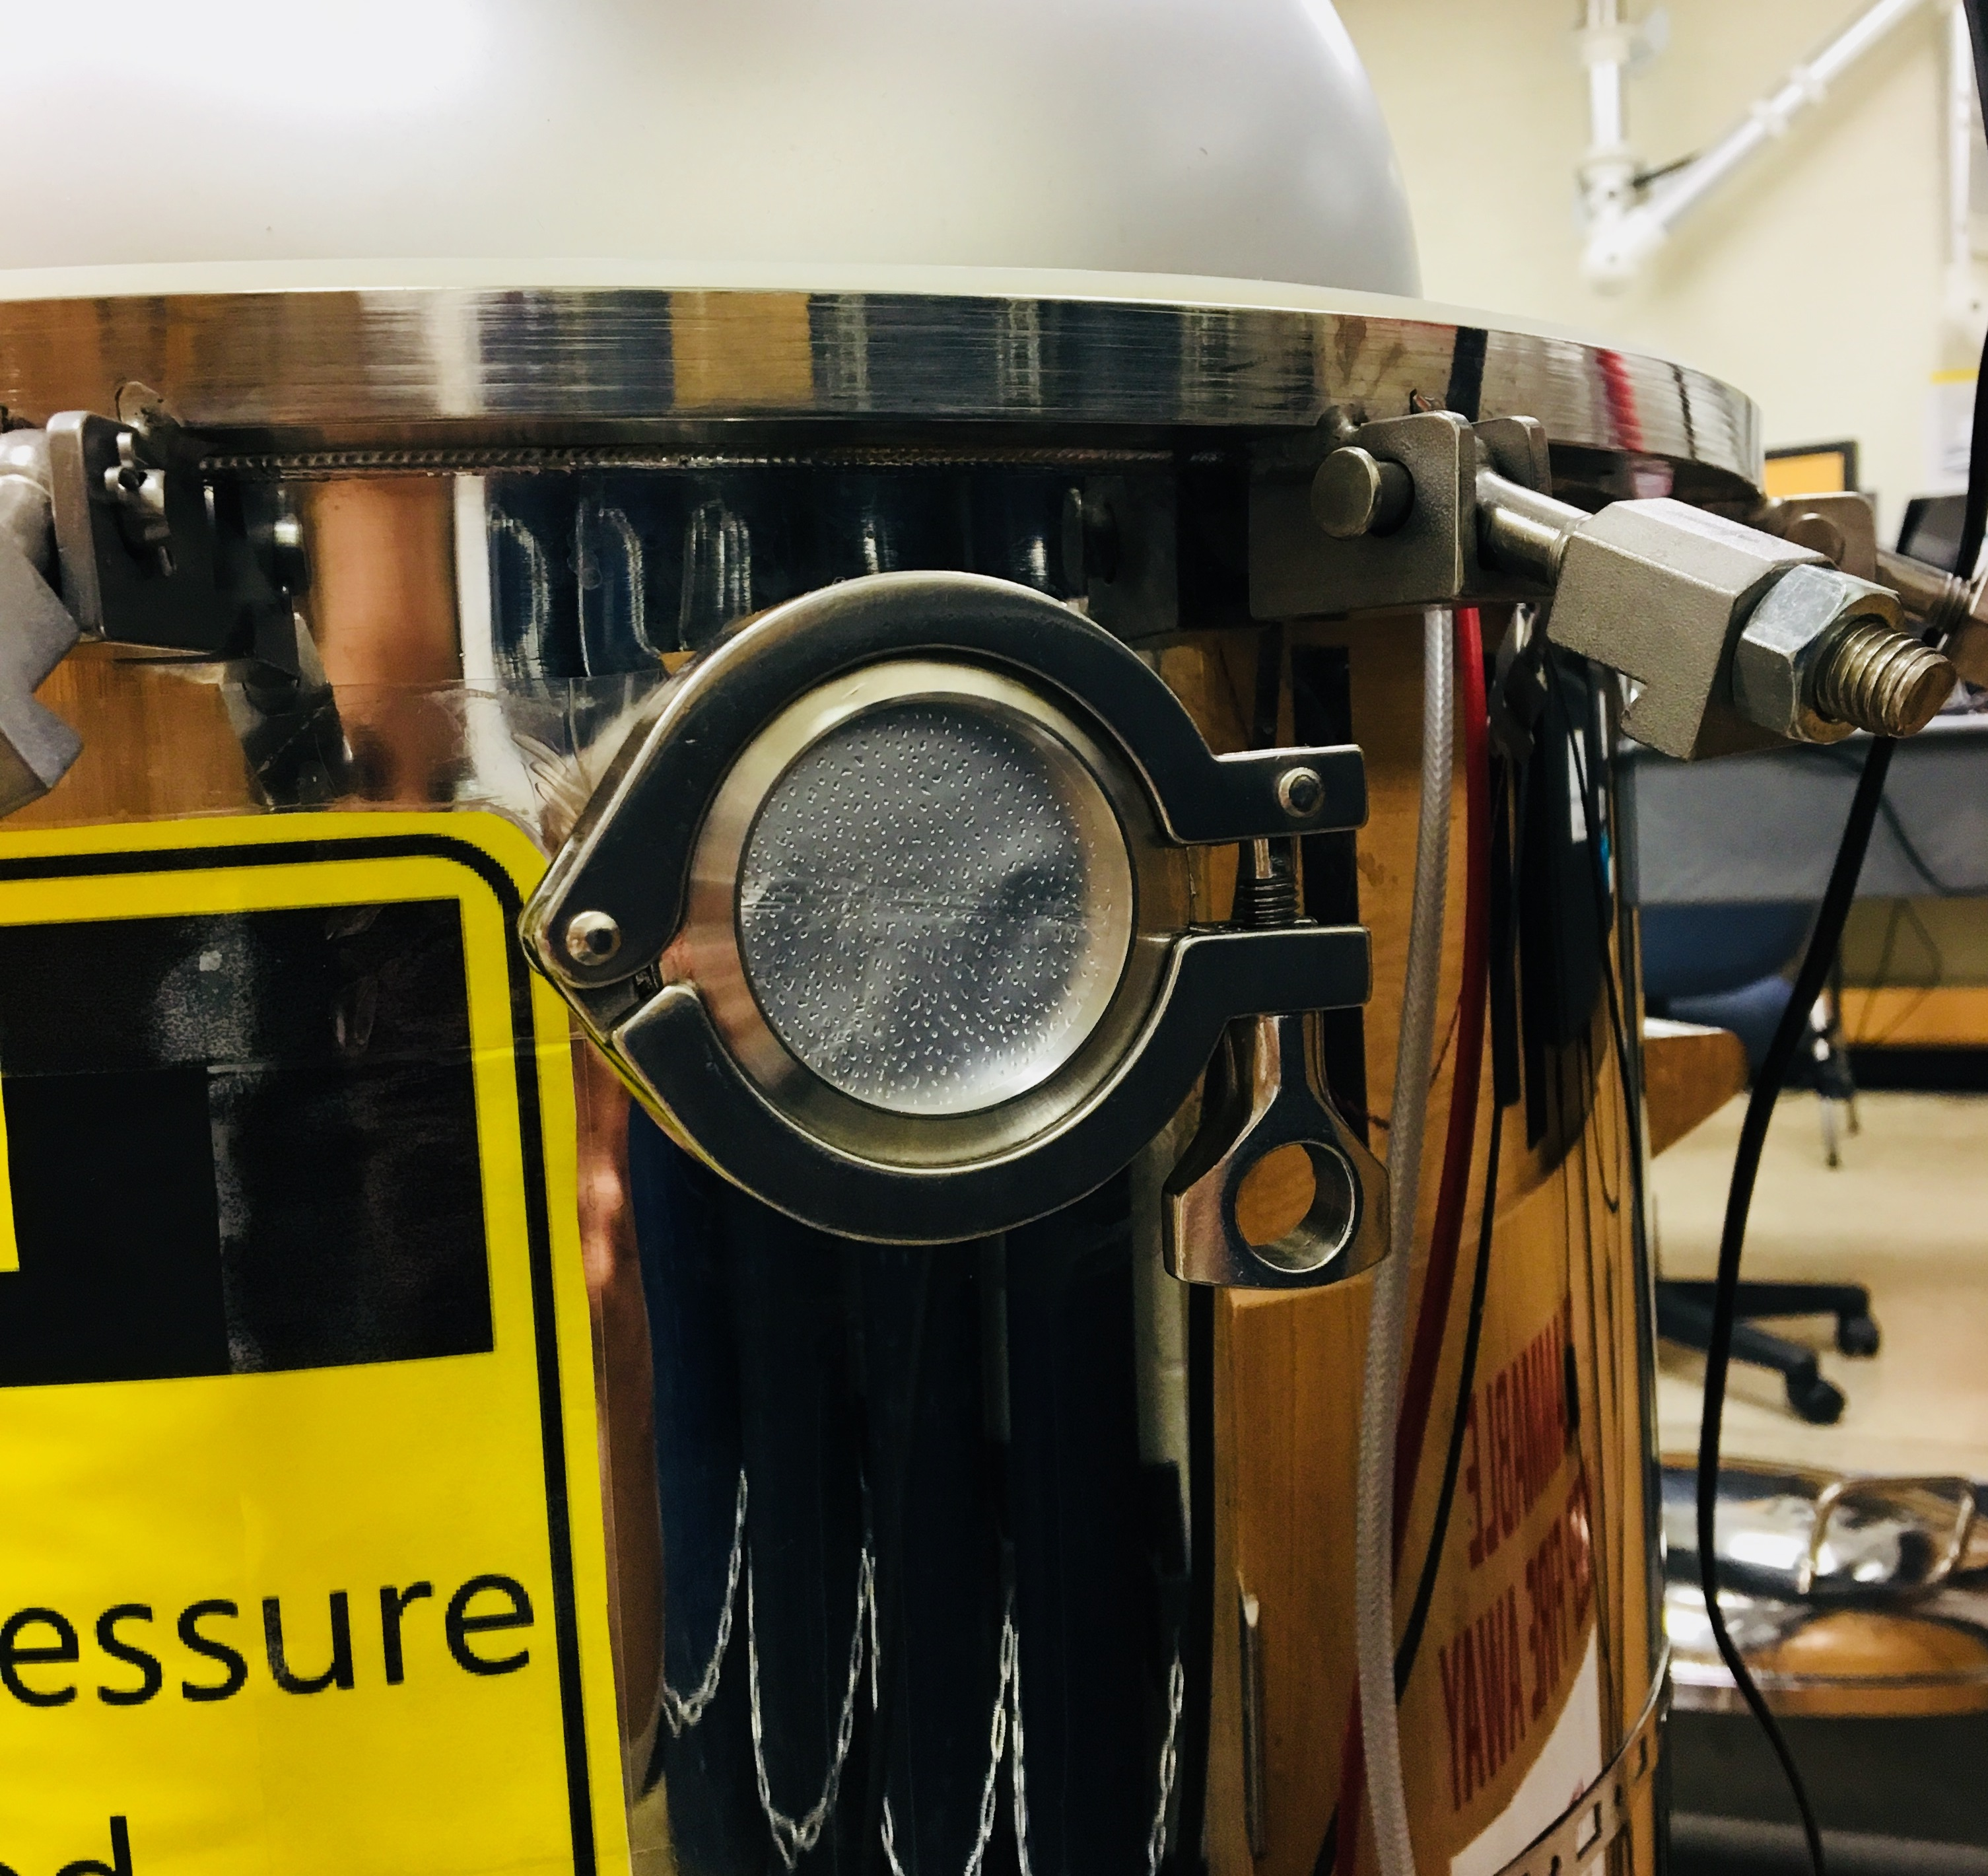
\includegraphics[width=0.5\textwidth]{./rupture_disk.jpg}
  \caption{Ensure the rupture disk is present and
  intact}\label{fig:rupture_disk}
  }
  \end{figure}
\item
  Start up computer and log on

  \begin{itemize}
  \tightlist
  \item
    Use the ``AIT Research Assistant'' account to log in

    \begin{itemize}
    \tightlist
    \item
      Username: aitra
    \item
      Password: hotflame16
    \end{itemize}
  \end{itemize}
\item
  Ensure a compatible SD card is inserted securely into the TADA
  datalogger (See Figure \ref{fig:sd_card_reader})

  \begin{figure}
  \hypertarget{fig:sd_card_reader}{%
  \centering
  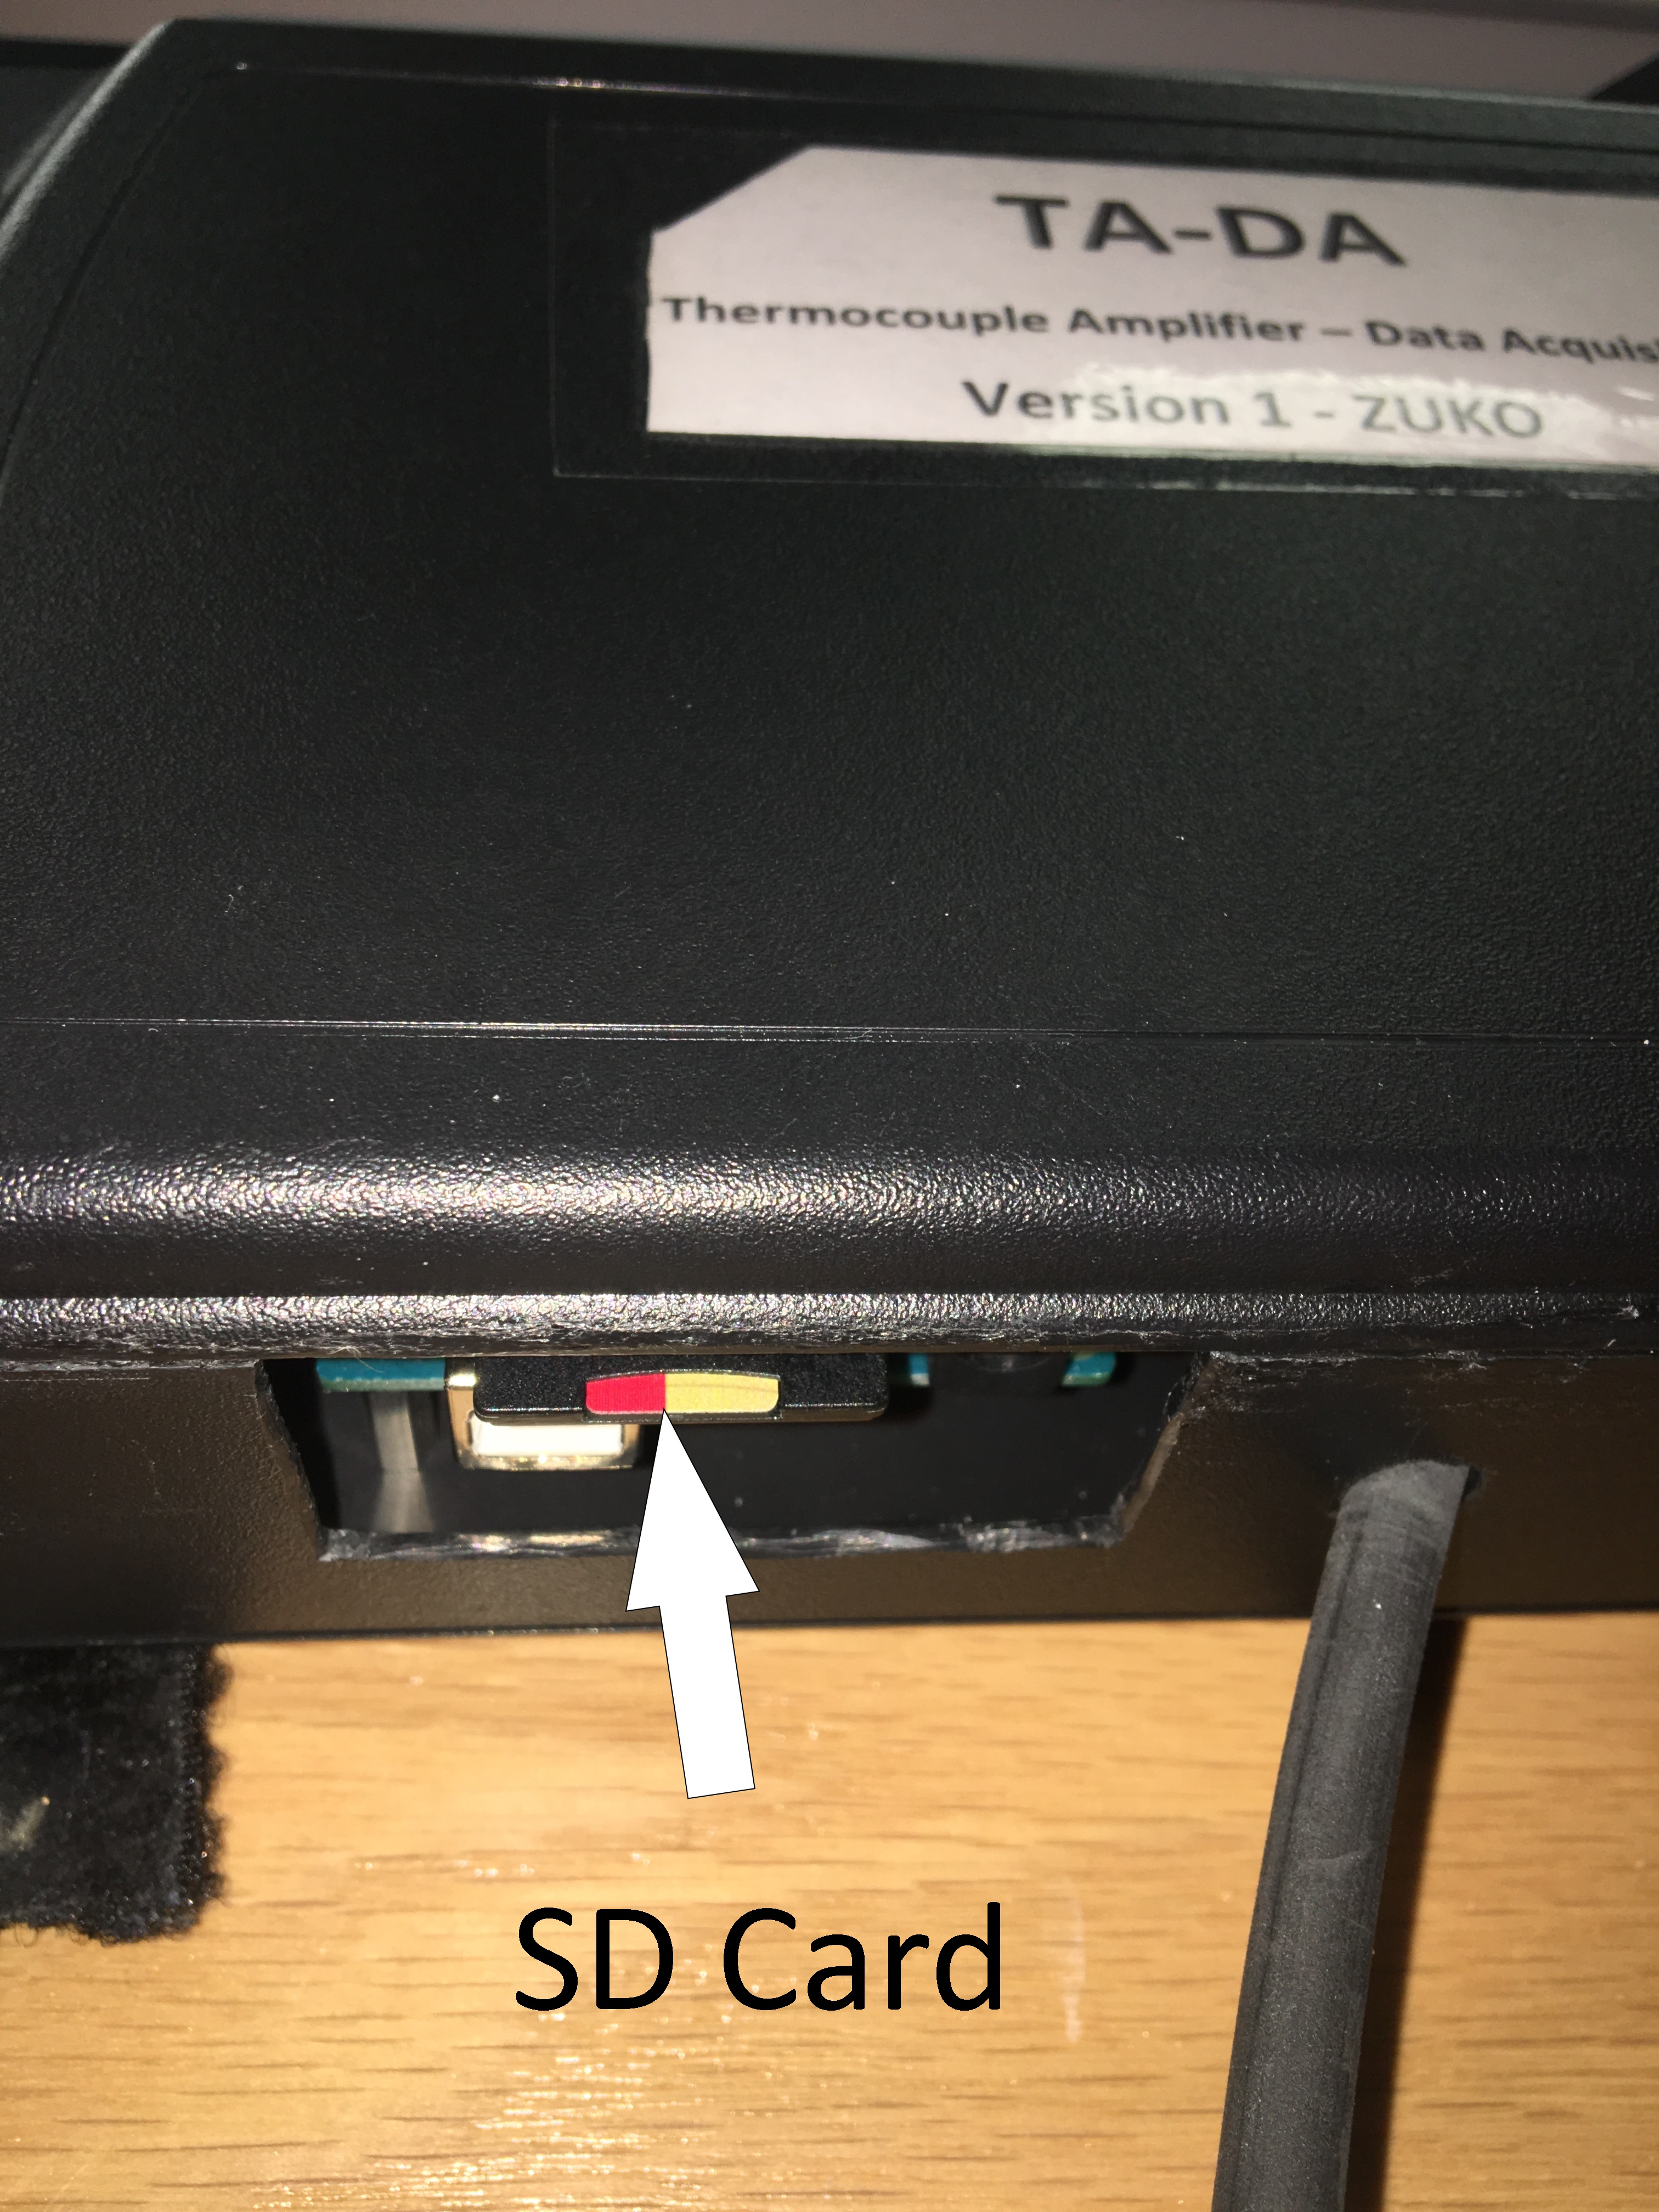
\includegraphics[width=0.5\textwidth]{./sd_card_reader.jpg}
  \caption{SD card slot location}\label{fig:sd_card_reader}
  }
  \end{figure}
\item
  Ensure the 4 furnace thermocouples are connected to their
  corresponding connectors inside the vessel and ensure that the wires
  are tucked down between the side of the furnace and the wall of the
  vessel and are out of the way (See Figure \ref{fig:Thermocouples})

  \begin{itemize}
  \item
    Thermocouple wires coming out of the furnace are numbered and should
    connect to the corresponding brown wire connected to the TADA

    \begin{figure}
    \hypertarget{fig:Thermocouples}{%
    \centering
    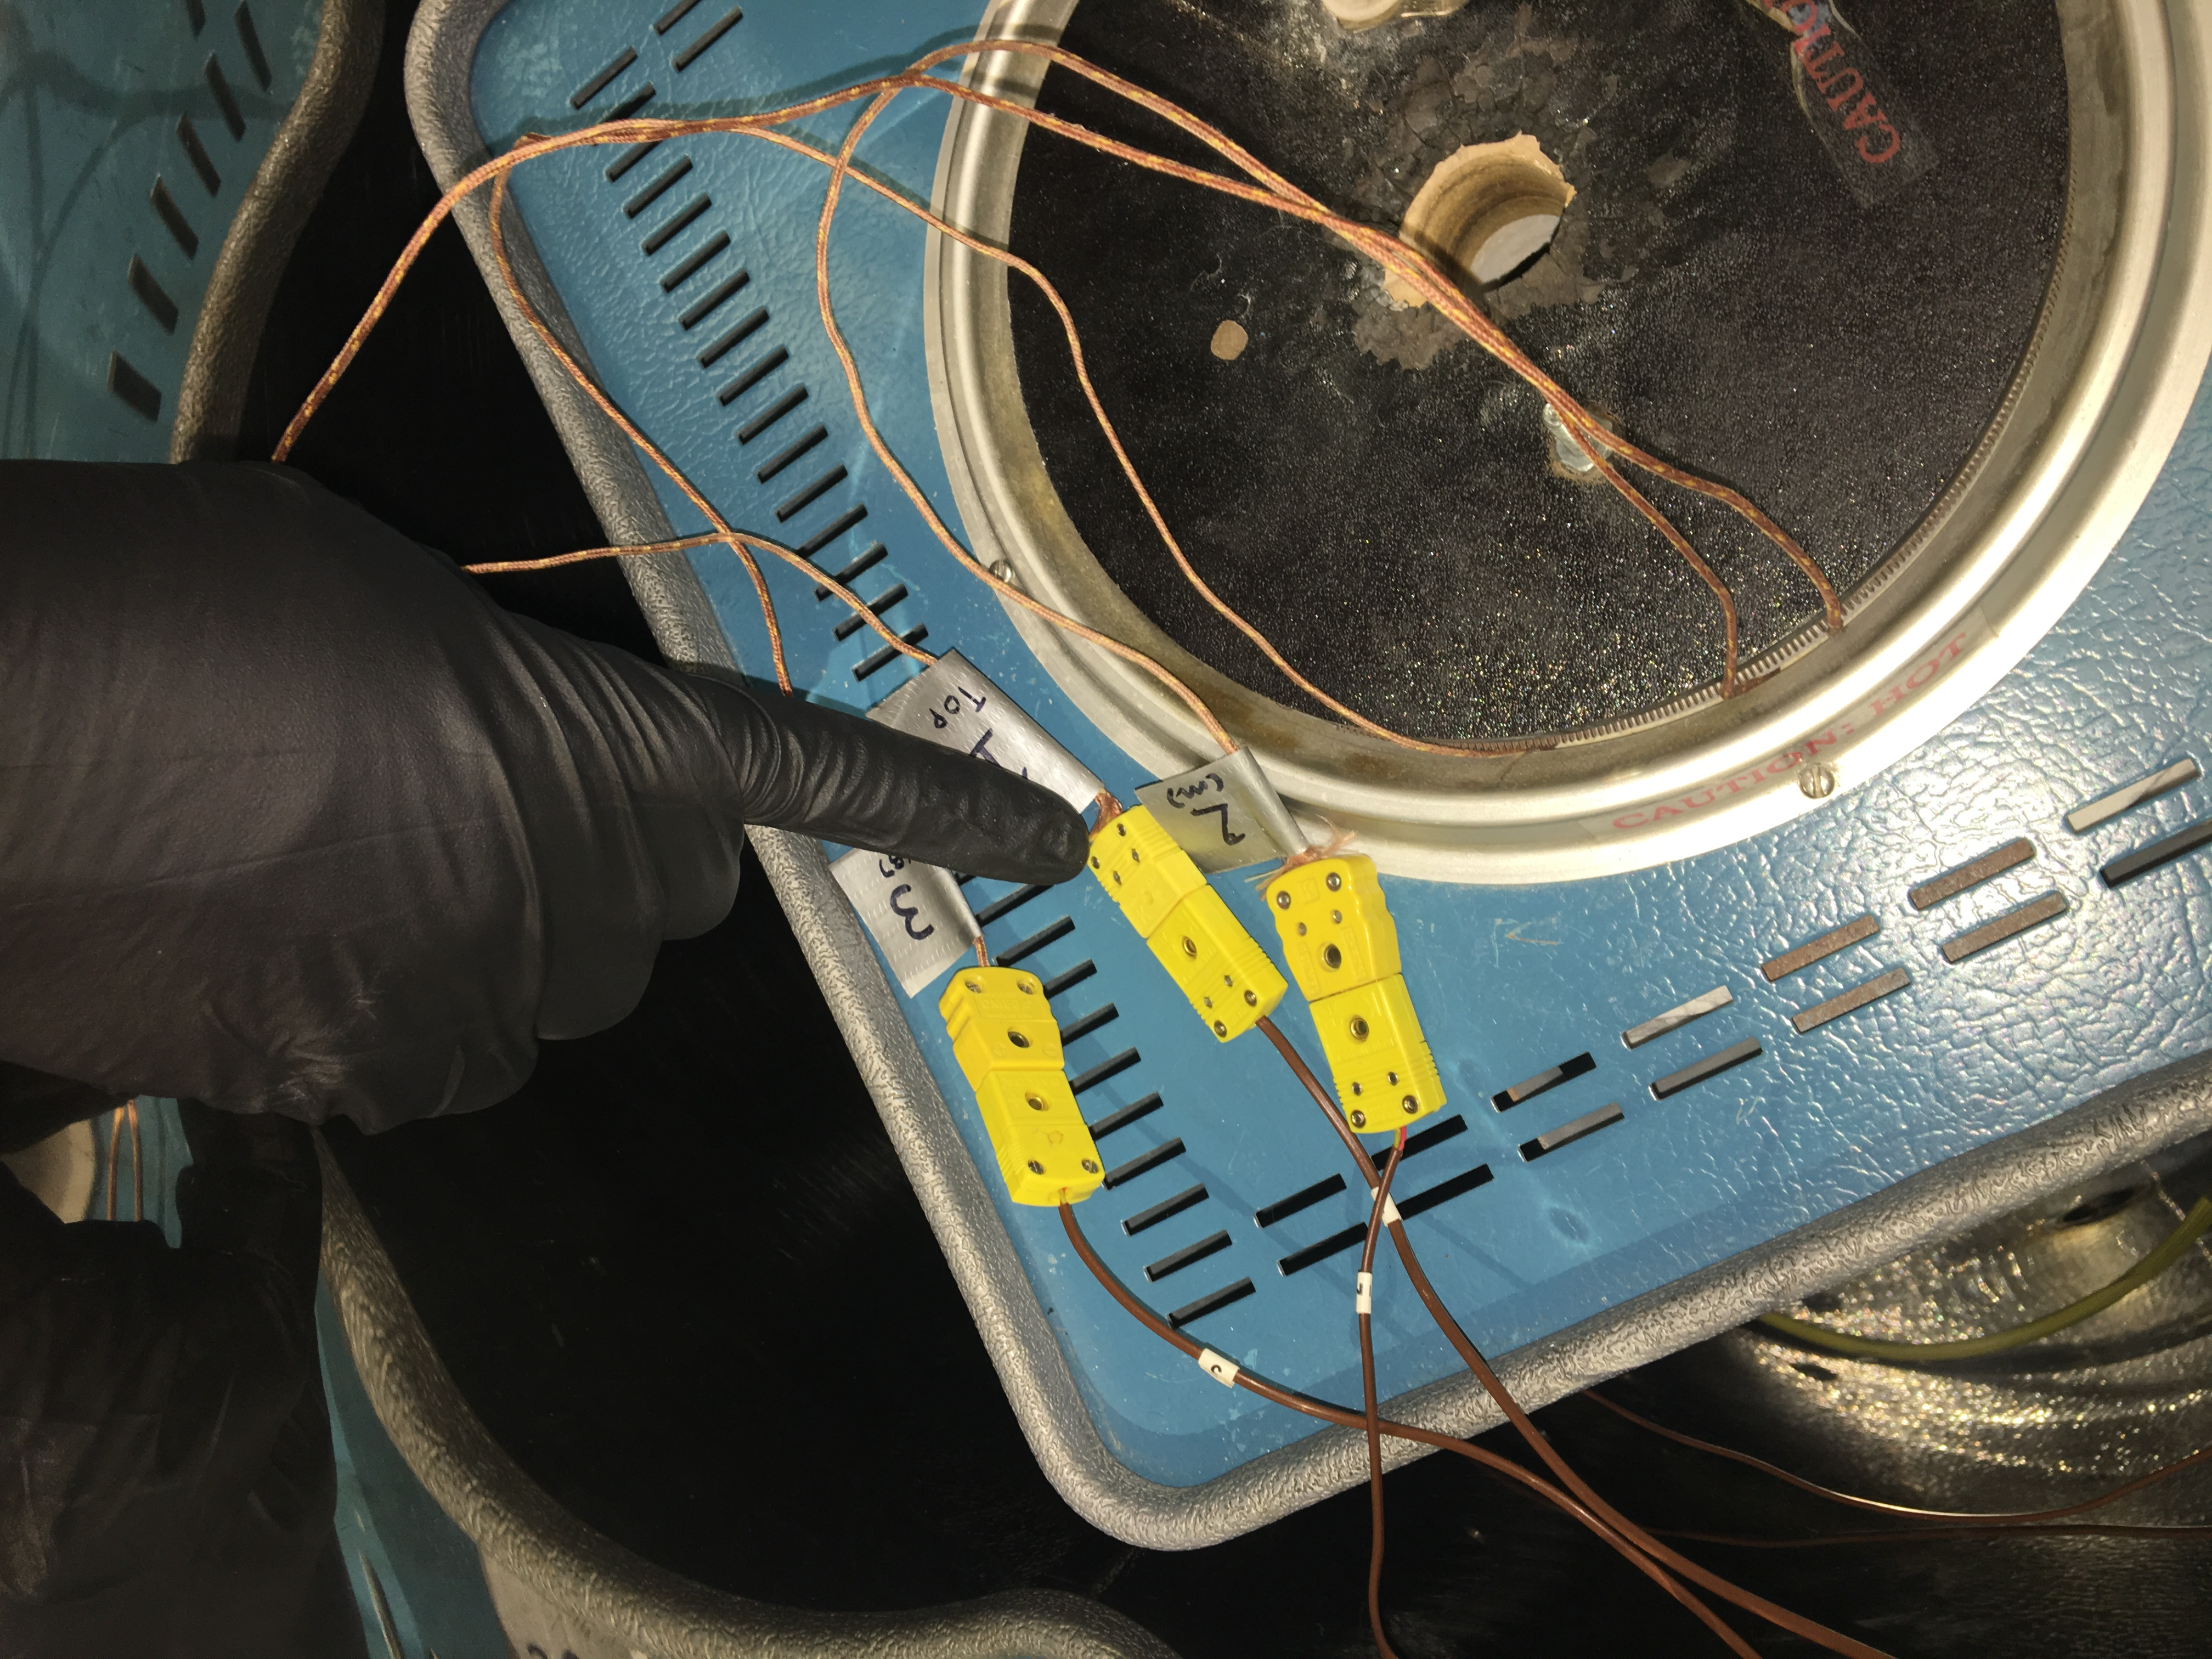
\includegraphics[width=0.5\textwidth]{./Thermocouples.jpg}
    \caption{Thermocouple connections}\label{fig:Thermocouples}
    }
    \end{figure}
  \end{itemize}
\item
  Connect the TADA to the lab computer via the USB cable mounted under
  the edge of the hood (see Figure \ref{fig:tada_connect})

  \begin{figure}
  \hypertarget{fig:tada_connect}{%
  \centering
  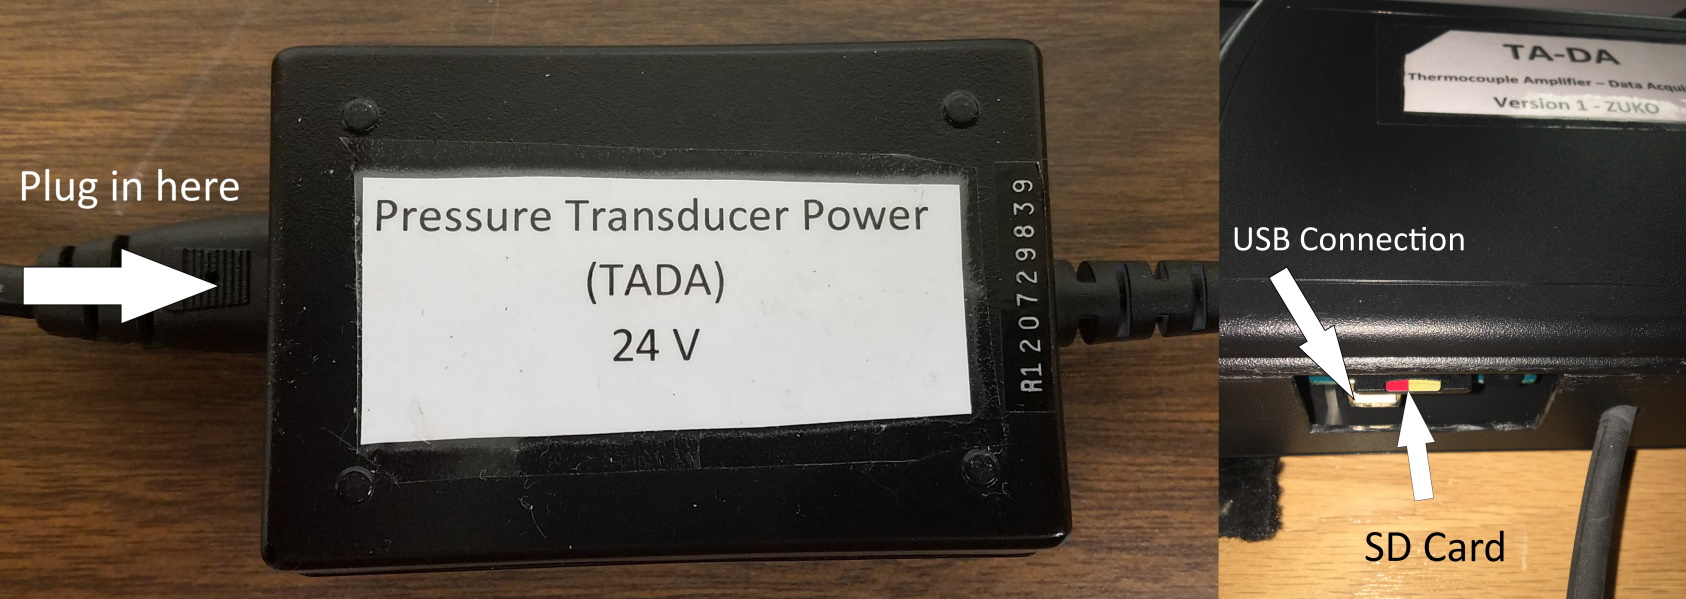
\includegraphics[width=0.5\textwidth]{./24v_powersupply.jpg}
  \caption{TADA Connections}\label{fig:tada_connect}
  }
  \end{figure}
\item
  Plug in the wall power to the TADA 24-volt power supply (see Figure
  \ref{fig:tada_connect})
\item
  Open the TADA user interface program

  \begin{itemize}
  \tightlist
  \item
    There should be a shortcut to this program on the desktop
  \item
    Path: \texttt{/home/aitra/Documents/ait\_exp/tada/tada\_main.py}
  \item
    The program will open two windows. \textbf{Ensure both windows are
    visible while using the program.}
  \item
    The serial communication LED in the TADA will start flashing
  \end{itemize}
\end{enumerate}

\begin{figure}
\hypertarget{fig:tada_leds}{%
\centering
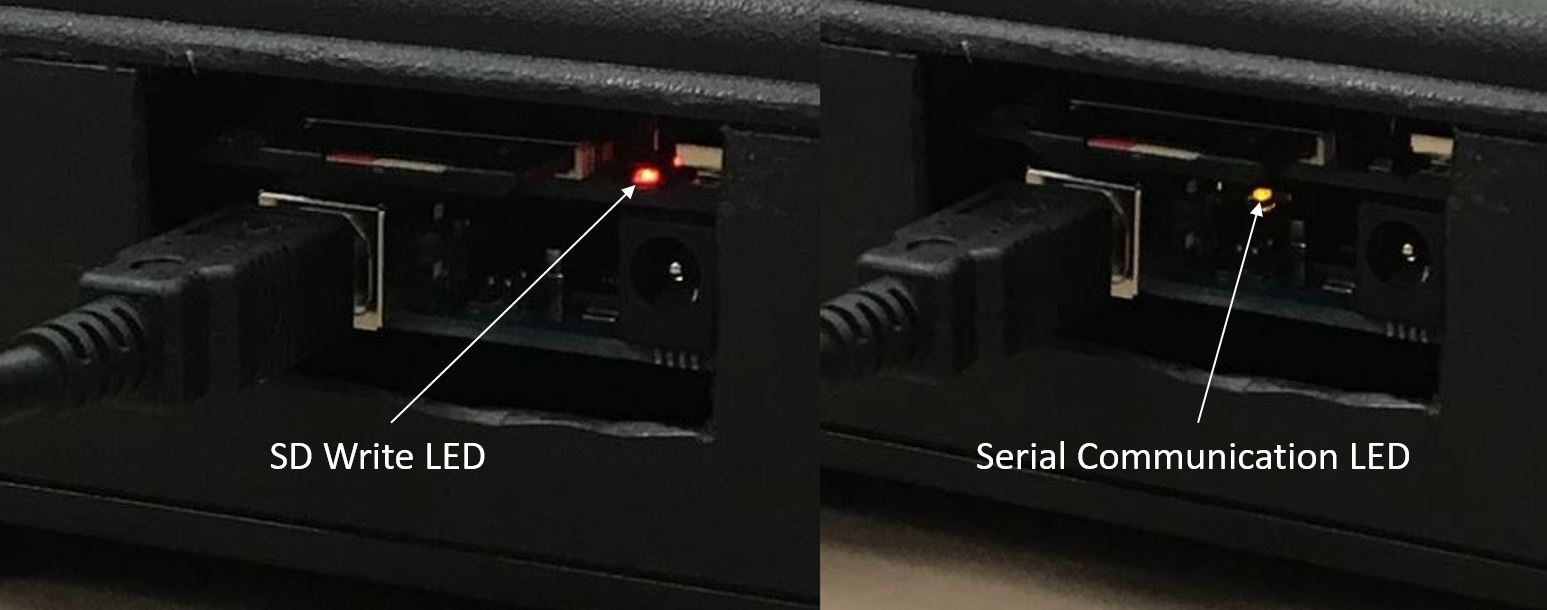
\includegraphics[width=0.5\textwidth]{./led_red_yellow.jpg}
\caption{Control LEDs inside the TADA}\label{fig:tada_leds}
}
\end{figure}

\begin{enumerate}
\def\labelenumi{\arabic{enumi}.}
\setcounter{enumi}{11}
\item
  Twist both of the ARIA lead screws by hand such that the mounting
  plate is all the way down and touching the base plate and the push
  block all the way back and is touching the horizontal stepper motor.
  (This is the shutdown position. See Figure
  \ref{fig:shutdown_position})

  \begin{figure}
  \hypertarget{fig:shutdown_position}{%
  \centering
  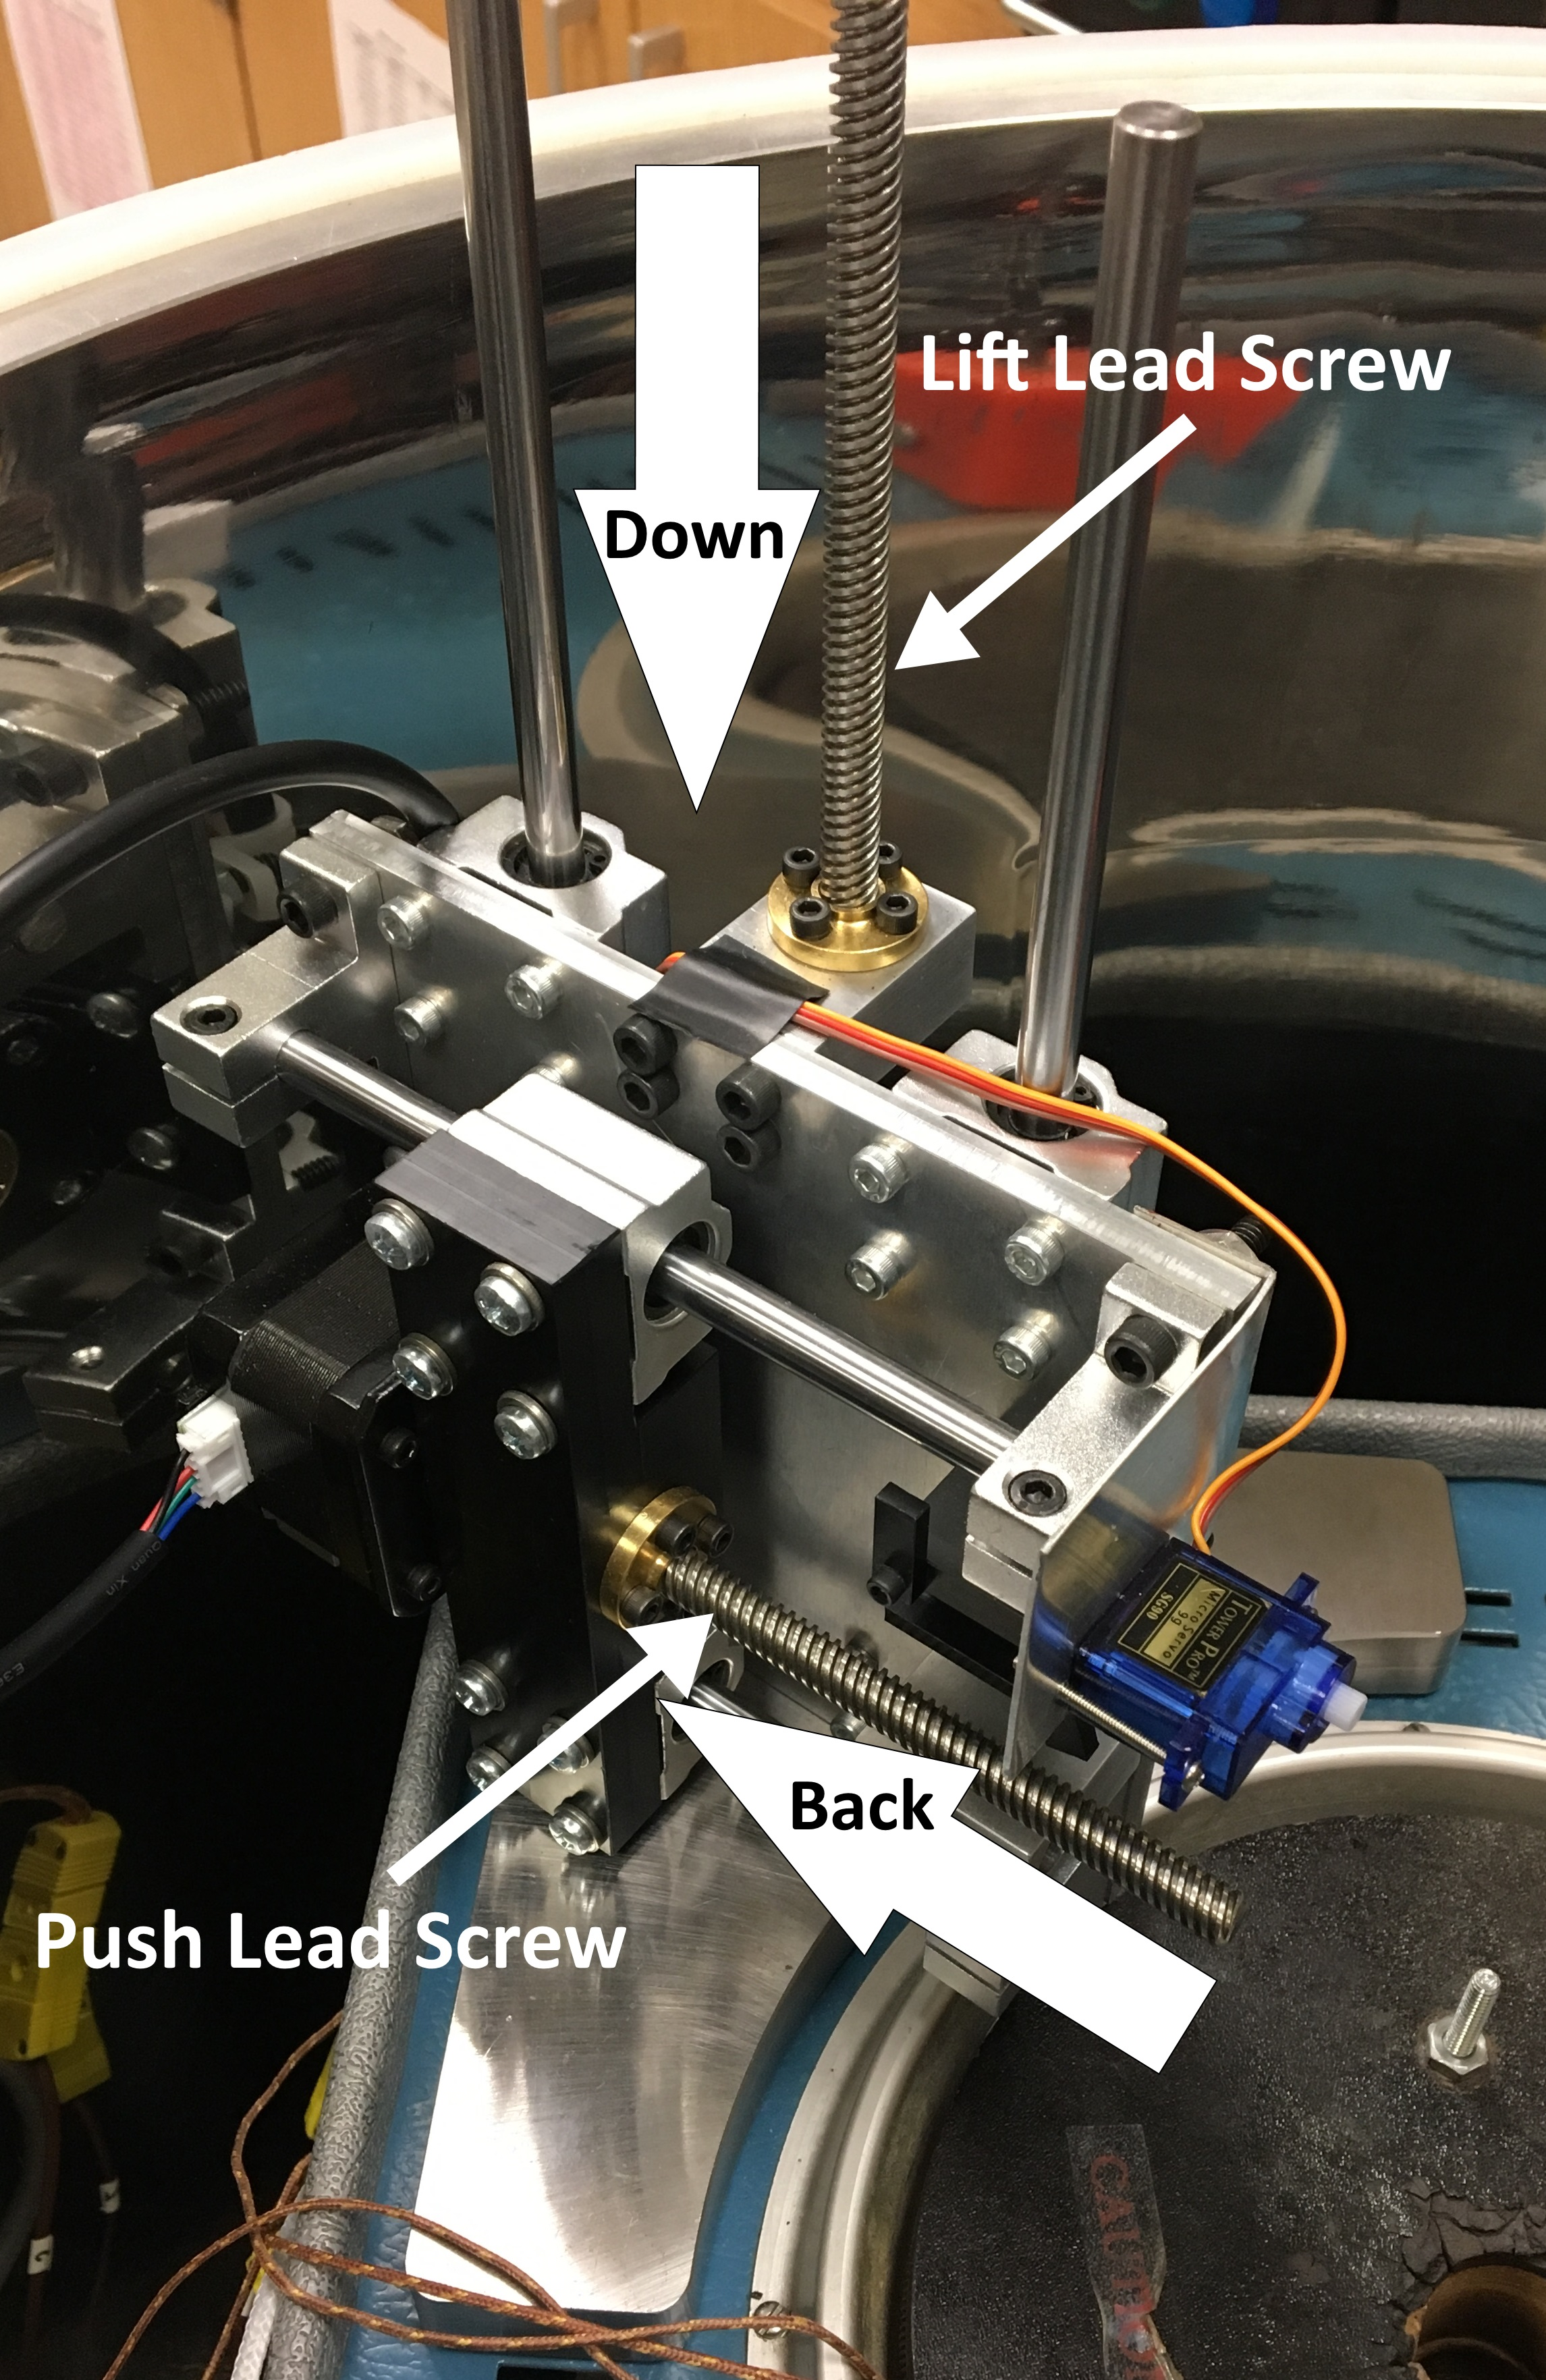
\includegraphics[width=0.5\textwidth]{./shutdown_position.jpg}
  \caption{The shutdown position for the
  ARIA}\label{fig:shutdown_position}
  }
  \end{figure}
\item
  Ensure the three molex cables are securely plugged in to the ARIA (see
  Figure \ref{fig:Molex_cables})

  \begin{itemize}
  \tightlist
  \item
    Regardless of the experiments to be performed, ensure all three are
    plugged in and the corresponding cables are not strained
  \end{itemize}

  \begin{figure}
  \hypertarget{fig:Molex_cables}{%
  \centering
  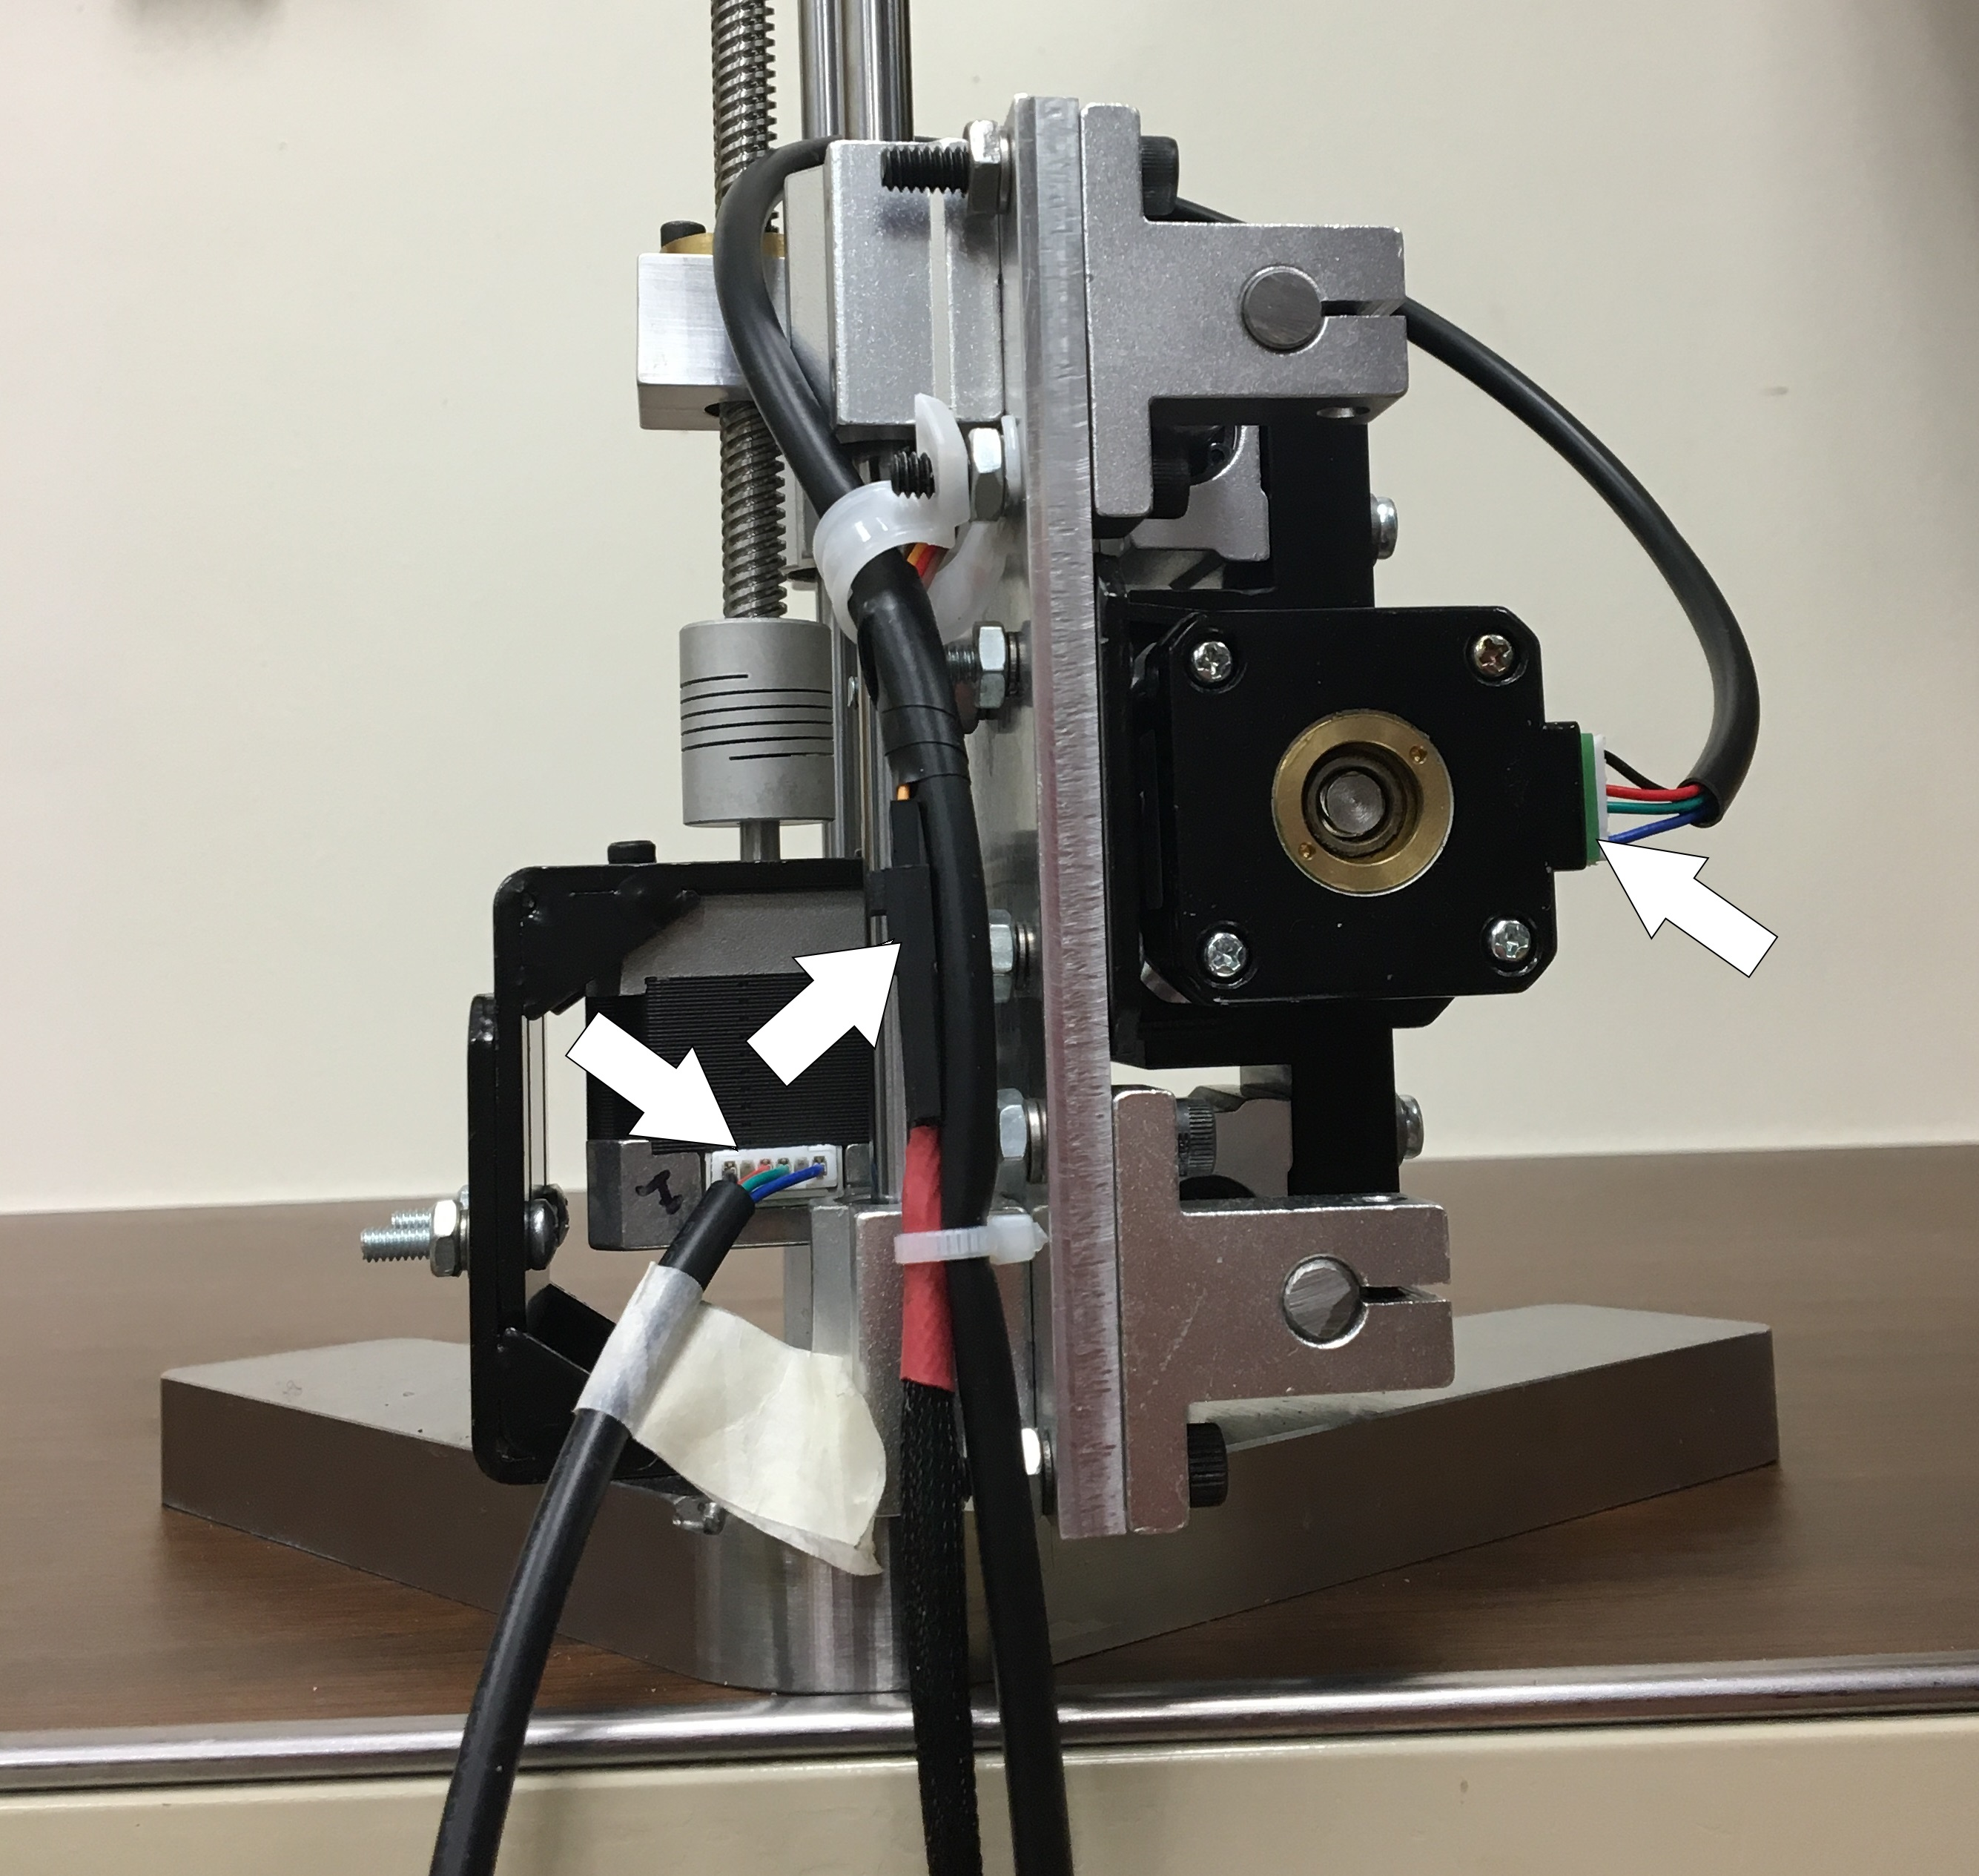
\includegraphics[width=0.5\textwidth]{./Molex_cables.jpg}
  \caption{Molex cables secured and out of the
  way}\label{fig:Molex_cables}
  }
  \end{figure}
\item
  Plug 5 volt power supply into the ARIA control and wait for initial
  setup sequence to complete (The two button lights on the ARIA control
  will come on when the sequence is complete) (See Figure
  \ref{fig:5V_cable})

  \begin{figure}
  \hypertarget{fig:5V_cable}{%
  \centering
  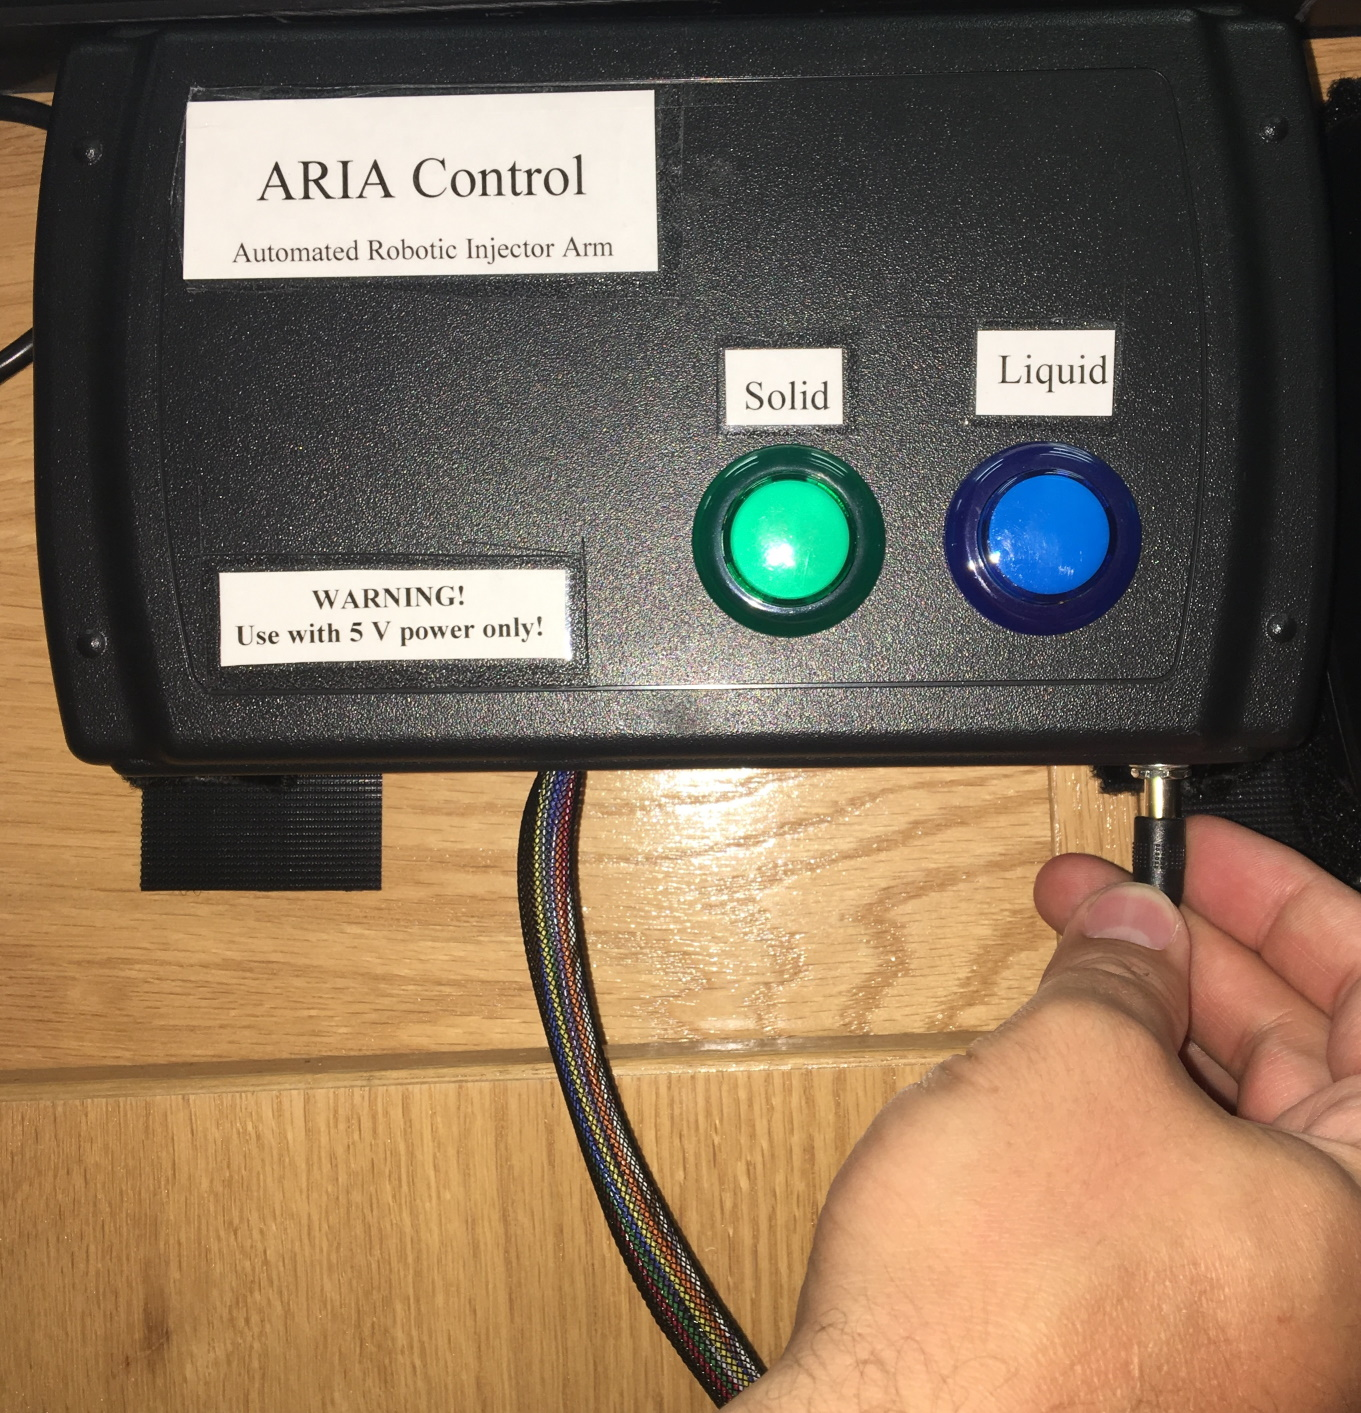
\includegraphics[width=0.5\textwidth]{./5V_cable.jpg}
  \caption{Plug in ARIA; 5V ONLY}\label{fig:5V_cable}
  }
  \end{figure}
\item
  Test the placement of the ARIA using the funnel and ring stand

  \begin{itemize}
  \item
    Use nitrile gloves when touching the ARIA
  \item
    Ensure the ring stand is secure in the ARIA, place the funnel in the
    ring stand and run the solid program (Press the ``Solid'' Button
    \textbf{without gloves on})
  \item
    Note that the end of the ring stand rod must be nearly flush with
    the inside surface of the ring stand mount block (See Figure
    \ref{fig:flush_r_stand})
  \item
    If the funnel does not go directly into the flask, adjust the
    placement and retest until properly positioned

    \begin{figure}
    \hypertarget{fig:flush_r_stand}{%
    \centering
    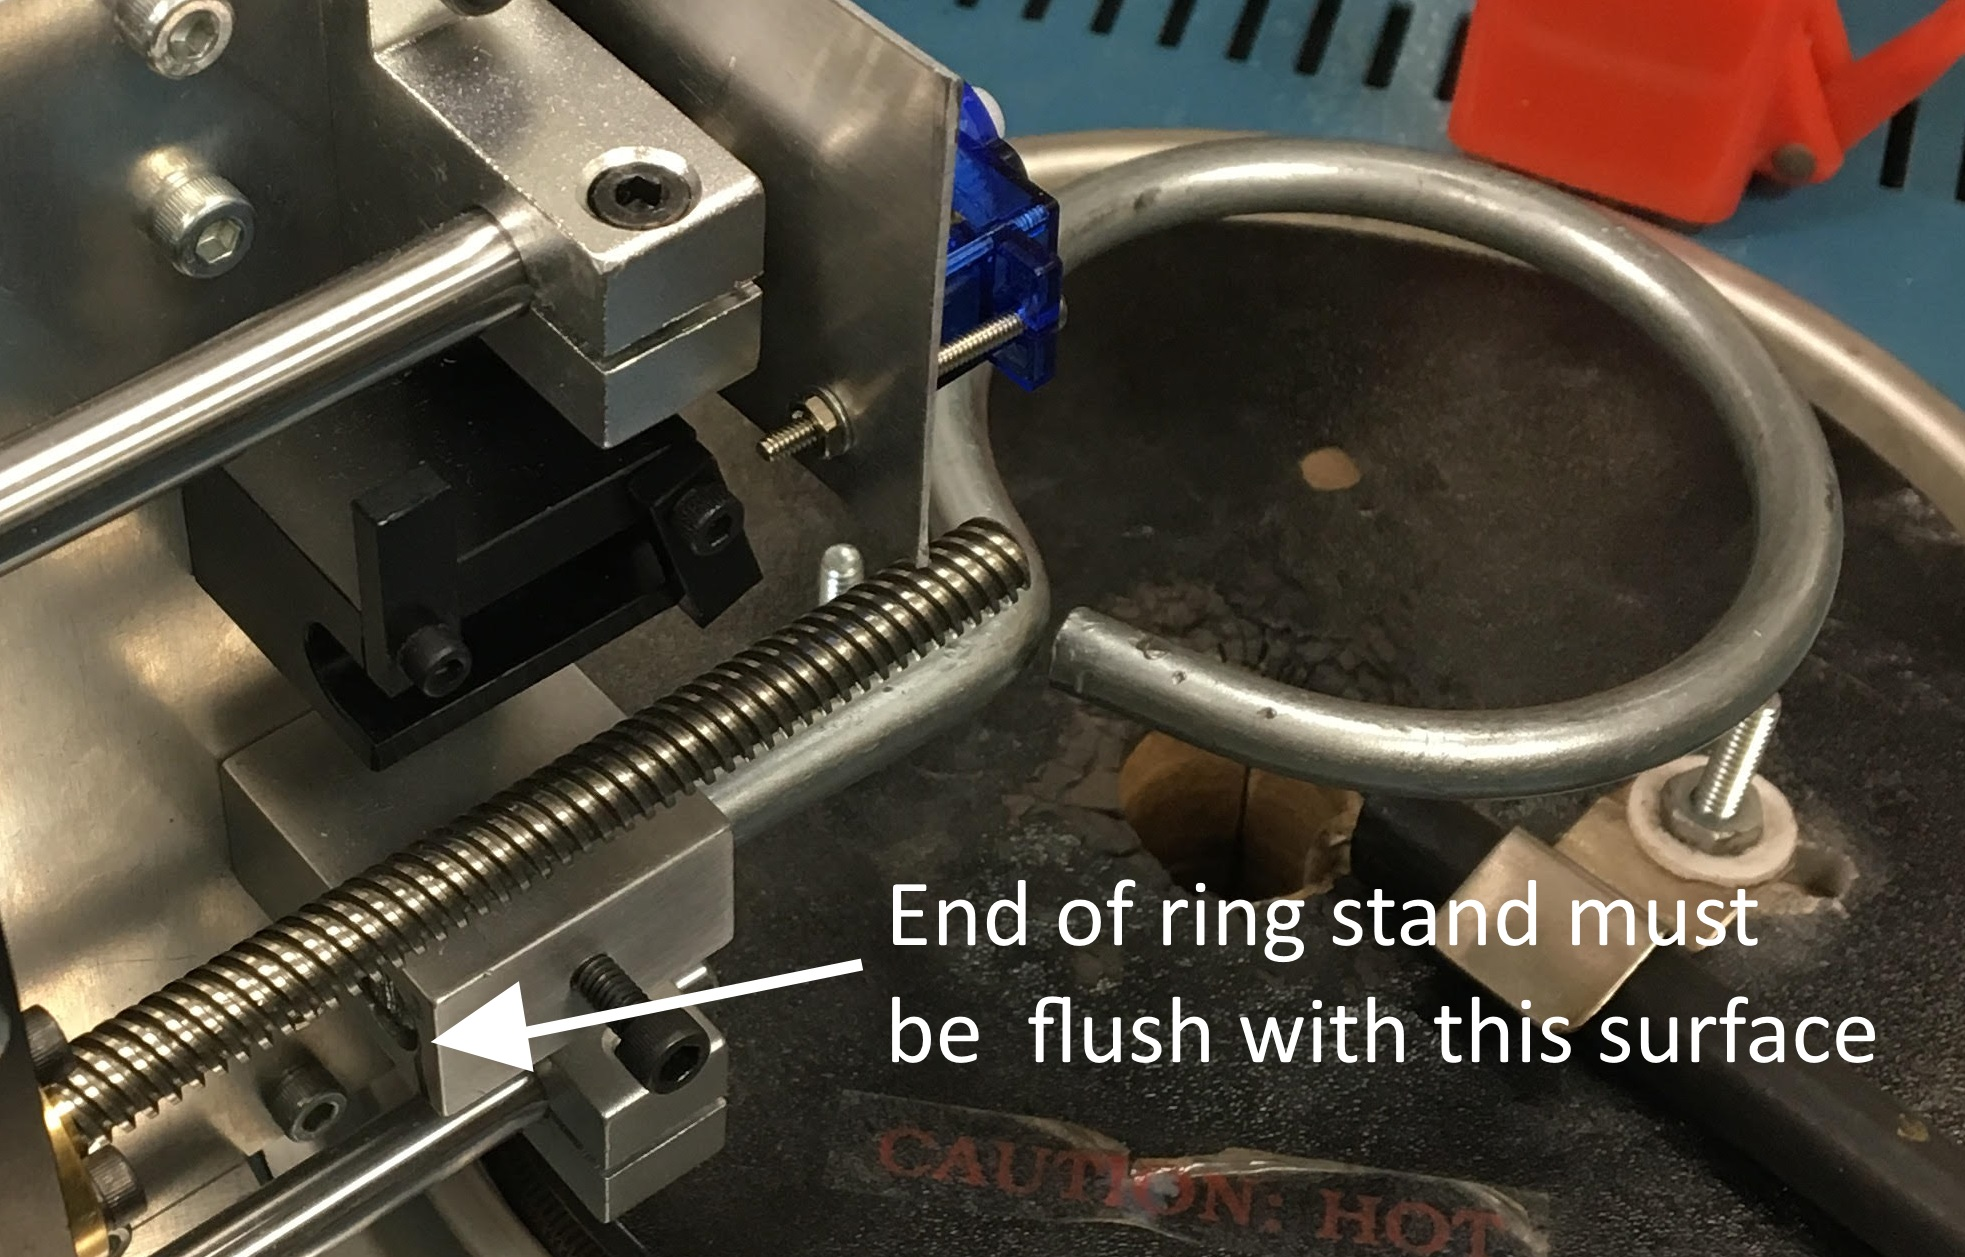
\includegraphics[width=0.5\textwidth]{./flush_r_stand.jpg}
    \caption{Place the ring stand so its end is flush with the inside
    surface of the mount block}\label{fig:flush_r_stand}
    }
    \end{figure}
  \end{itemize}
\item
  Test the placement of the mirror using the Camera Suite app and camera

  \begin{itemize}
  \tightlist
  \item
    Connect the computer to the camera's Wi-Fi (See Section
    refsec:cam\_tab on how to do this)
  \item
    Open the Camera Suite app to use the camera's view finder
  \item
    Mount the camera on the side of the furnace (See Section
    refsec:cam\_on\_furn)
  \item
    Using the camera's view finder, adjust the position of the mirror on
    the furnace to align the camera's view to see directly down the
    center of the flask
  \item
    The camera should be positioned so that the hole in the furnace and
    the mirror are visible
  \item
    Once you have aligned the mirror, remove and shutdown the camera for
    initial furnace heating
  \end{itemize}
\item
  Check the glass wool air filter in the inlet of the rotameter replace
  if necessary (See Section ???)
\item
  Once the target temperature is reached, allow the system to come to
  equilibrium

  \begin{itemize}
  \tightlist
  \item
    The ``Temp Ready'' indicator in the TADA\_UI window should turn
    green when the system has come to an acceptable equilibrated state
  \item
    Sometimes the ``Temp Ready'' indicator may not turn green if the
    flask was not installed correctly (See Section
    \ref{sec:Flask-and-Lid}) or there are problems with the
    thermocouples even when the flask has reached thermal equilibrium.
    Therefore, while heating up or changing temperatures, check the
    temperatures that are displayed in the command line window of the
    TADA\_UI. If the temperatures are not within about 20 K of each
    other the thermocouples may not be placed properly. If this is the
    case experiments may proceed as normal but thermal equilibrium must
    be verified manually by using the data on the command line window
    and neglecting the misplaced thermocouple.
  \item
    If any of the thermocouples in the command line window of the
    TADA\_UI read ``NAN'' (not a number) then that thermocouple is not
    connected. Check all thermocouple connections and reconnect the
    thermocouple if possible.
  \end{itemize}
\end{enumerate}

\hypertarget{experimental}{%
\subsection{Experimental}\label{experimental}}

This section outlines the steps for experimental runs. Each experiment
should be performed following these steps exactly (insofar as that is
possible). Doing so will ensure consistent results with the lowest
uncertainty possible.

\hypertarget{pre-experimental-safety-checks}{%
\subsubsection{Pre-Experimental Safety
Checks}\label{pre-experimental-safety-checks}}

Before beginning experiments, ALL operators must do the following:

\begin{itemize}
\tightlist
\item
  Ensure your workspace, the area around the computer and both hoods are
  free of clutter, tripping hazards or anything which could present a
  hazard to you or anyone else in the lab
\item
  Review Safety Data Sheets (SDS) and understand all hazards presented
  by all compounds that will be handled

  \begin{itemize}
  \tightlist
  \item
    This needs to be done only once before handling each compound for
    the first time but, SDS's should be reviewed periodically
  \item
    All chemical handling should be done in the hood whenever possible.
    The main exceptions to this rule are for injection into the furnace
    and using the mass balance.
  \item
    Refer to the compound's SDS for specific recommendations on chemical
    handling
  \end{itemize}
\item
  Ensure you are using appropriate PPE for handling chemicals
  (e.g.~nitrile gloves and splash goggles)

  \begin{itemize}
  \tightlist
  \item
    Refer to the SDS for the chemical you are working with when
    determining appropriate PPE
  \item
    NOTE: Some SDS's will recommend using a face shield in addition to
    splash goggles when handing their respective chemicals. In our lab
    we will use ventilation hoods which, when used properly, serve as
    better protection than face shields. Therefore, any time an SDS
    recommends using a face shield you may safely ignore that
    recommendation provided you are using the hood properly by
    positioning the sash between your face and the work being performed
    in the hood.
  \item
    Unless an SDS states otherwise, lab coats are recommended but not
    required when handling chemicals
  \end{itemize}
\end{itemize}

\hypertarget{experimental-procedure-steps}{%
\subsubsection{Experimental Procedure
Steps}\label{experimental-procedure-steps}}

\begin{enumerate}
\def\labelenumi{\arabic{enumi}.}
\item
  Measure out sample

  \begin{itemize}
  \item
    Liquids

    \begin{itemize}
    \tightlist
    \item
      Before measuring a sample out for the first time, clean the
      syringe of any residual compound

      \begin{enumerate}
      \def\labelenumii{\arabic{enumii}.}
      \tightlist
      \item
        Take 2 clean 100 ml beakers and put them in the hood (these will
        be your sample and waste beakers)
      \item
        Place a small amount of compound into the sample beaker
      \item
        Rinse the syringe of any extraneous compounds 3 times by drawing
        approximately 300 microliters into the syringe from the sample
        beaker and eject it into the waste beaker
      \end{enumerate}
    \item
      Draw sample amount into a right-angle syringe

      \begin{enumerate}
      \def\labelenumii{\arabic{enumii}.}
      \tightlist
      \item
        Begin by drawing an excess amount of compound into the syringe
      \item
        Draw slowly to minimize air bubbles in the syringe
      \item
        Hold syringe vertically to move air bubbles to the top, gently
        tapping the syringe if necessary
      \item
        Carefully eject the syringe into the waste beaker to remove any
        air bubbles until the syringe reads the desired amount
      \end{enumerate}
    \item
      The final sample size should not exceed 250 microliters
    \end{itemize}
  \item
    Solids

    \begin{itemize}
    \tightlist
    \item
      Measure out sample on a weigh boat

      \begin{enumerate}
      \def\labelenumii{\arabic{enumii}.}
      \tightlist
      \item
        Open the scale door by pressing the button with an asterisk '*'
        and place a new and empty weigh boat on the center of the scale
        plate
      \item
        Close the scale door with the asterisk button, and tare the
        scale
      \item
        Remove the weigh boat before measuring out sample
      \item
        Using a clean chemical spatula, scoop the desired amount from
        the compound container to the weigh boat, replacing the weigh
        boat on the scale to check until the desired mass is reached
      \item
        Take note of the initial mass of the compound sample (the mass
        should exceed the desired mass by about 10 mg)
      \item
        With the sample and weigh boat on the scale, tare the scale
      \item
        Remove the weigh boat from the scale
      \end{enumerate}
    \item
      The initial sample size should not exceed 300 mg
    \end{itemize}
  \item
    Gases

    \begin{itemize}
    \tightlist
    \item
      Draw sample amount into a right-angle syringe\\
    \item
      Sample size should not exceed 250 microliters
    \end{itemize}
  \end{itemize}
\item
  Secure the sample to the ARIA

  \begin{itemize}
  \item
    Liquid/Gases Sample

    \begin{enumerate}
    \def\labelenumii{\arabic{enumii}.}
    \tightlist
    \item
      Place the syringe securely into the syringe holder on the ARIA,
      making sure the needle is in the funnel
    \item
      Test placement one more time to ensure the funnel is guided into
      the injection hole (use the \textbf{solid} button)
    \end{enumerate}
  \item
    Solid Sample

    \begin{enumerate}
    \def\labelenumii{\arabic{enumii}.}
    \tightlist
    \item
      Carefully insert the weigh boat into the weigh boat holder sliding
      the securing wires out of the way as needed
    \item
      Gently tap the side of the weigh boat so that the sample collects
      in a pile near the leading corner of the weigh boat
    \item
      Press the weigh boat holder onto the servo shaft so the weigh boat
      is in a near-horizontal position
    \item
      Test placement one more time to ensure the funnel is guided into
      the injection hole (use the \textbf{liquid} button)
    \end{enumerate}
  \end{itemize}
\item
  Remove gloves before proceeding
\item
  Ensure the camera battery sufficiently charged and the camera is
  powered on

  \begin{itemize}
  \tightlist
  \item
    Reconnect the camera to the tablet if necessary
  \end{itemize}
\item
  Secure the camera to the side of the furnace

  \begin{itemize}
  \tightlist
  \item
    \textbf{Note for unpressurized experiments:} If you are performing
    unpressurized experiments (i.e.~experiments with the lid off) you
    may safely skip the next \textbf{three} steps. Before proceeding,
    ensure that the vessel is being vented by the snorkel.
  \end{itemize}
\item
  \textbf{Simultaneously} remove the snorkel from inside the vessel and
  place above the rupture disk (see Figure fig:rupture\_hood) textbfand
  place lid on pressure vessel and secure in place with the clamps and
  cable

  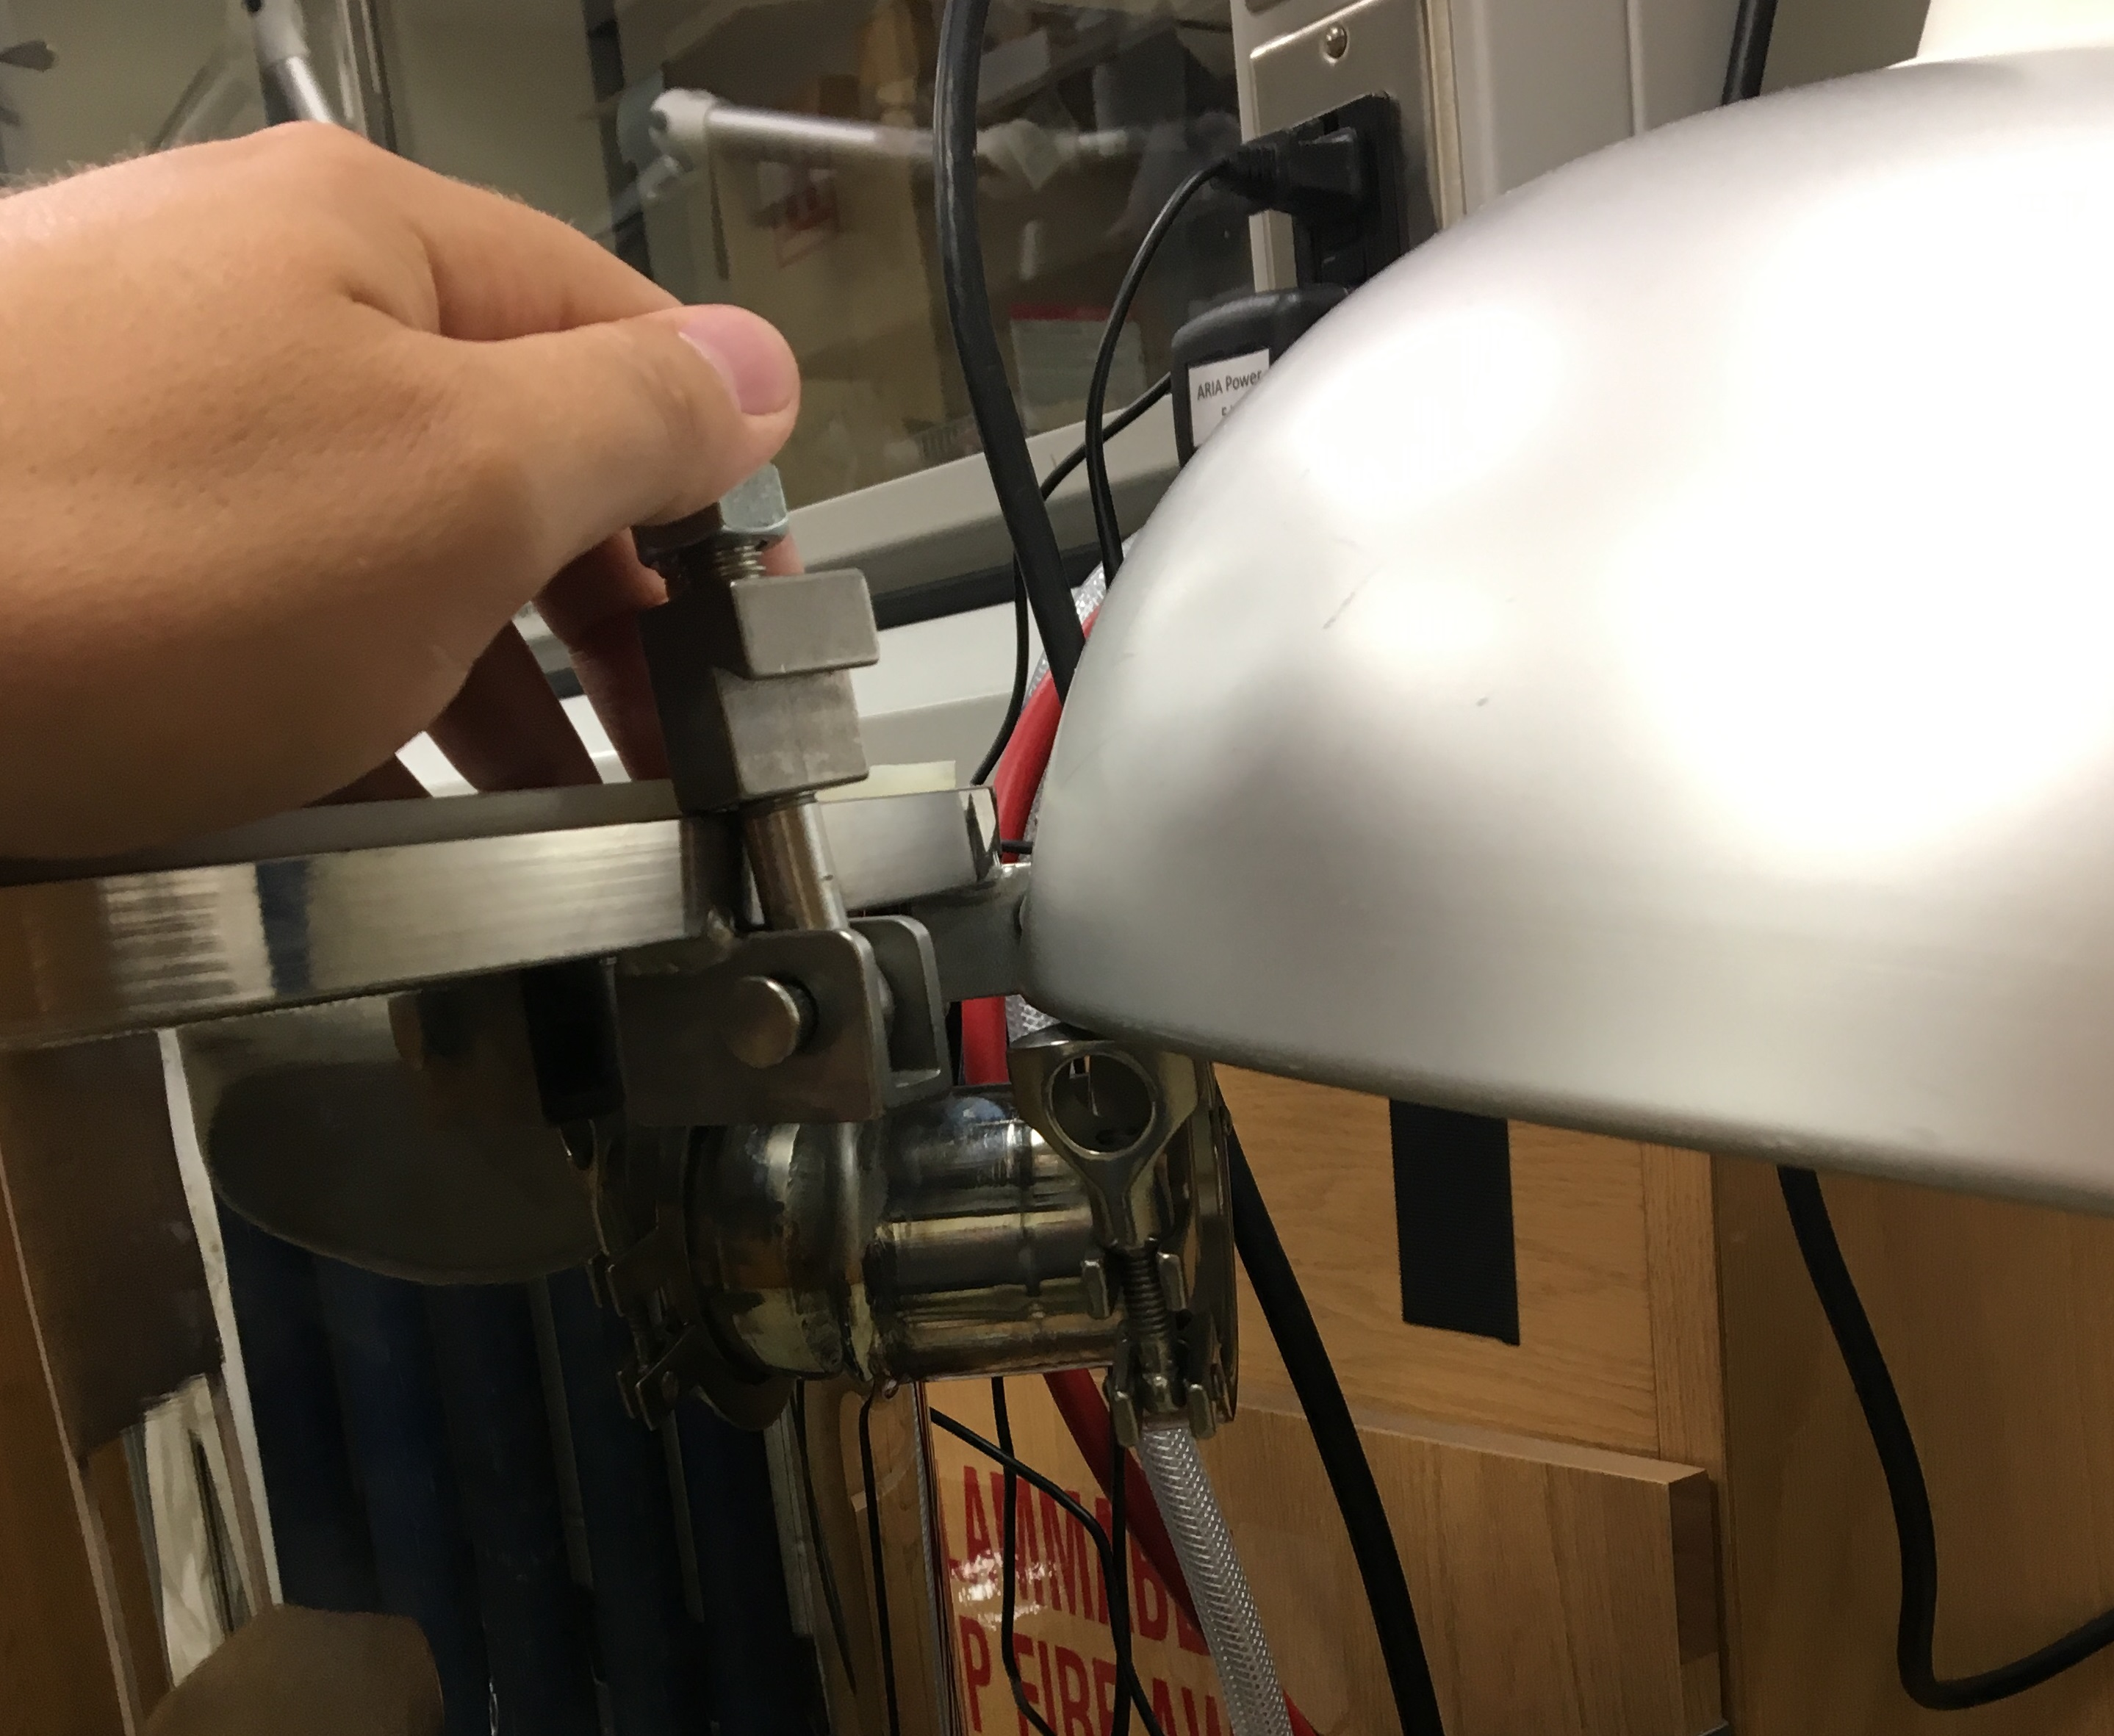
\includegraphics[width=0.5\textwidth]{./rupture_hood.jpg}Snorkel placement during
  operation\{\#fig:rupture\_hood --\textgreater{}

  \begin{itemize}
  \tightlist
  \item
    Two people are required to perform this step. One to remove the
    snorkel (Person B) and the other to place the lid (Person A)
  \end{itemize}

  \begin{enumerate}
  \def\labelenumii{\arabic{enumii}.}
  \tightlist
  \item
    Person A: open the sash on the hood vertically and carefully pull
    out the vessel lid ensuring the outlet hose does not catch on
    anything (do not pull it through the sliding doors)

    \begin{itemize}
    \tightlist
    \item
      Use caution when handling the lid; the lid is heavy
    \end{itemize}
  \item
    Person B: Lift up the bell on the snorkel so it can swing away from
    the open pressure vessel
  \item
    Person A and B: Simultaneously, place the lid on the vessel and
    swing the snorkel away from the vessel. This should be done in one
    simultaneous motion.
  \item
    Person B: Place the snorkel over the rupture disk as seen in Figure
    fig:rupture\_hood.

    \begin{itemize}
    \tightlist
    \item
      \textbf{The rest of the procedure requires only 1 person}
    \end{itemize}
  \item
    When placing the lid, hold the lid directly above the vessel and
    carefully lower it straight down on the vessel to avoid hitting the
    ARIA with the lid. Make sure to avoid crimping the outlet hose and
    keep it as smooth and straight as possible
  \item
    Line up the two marks on the lid with the corresponding marks on the
    vessel
  \item
    Ensure the lid is centered on the vessel by running your fingers
    around the edge to ensure the edge of the vessel and the lid are
    flush
  \item
    Check that the lid lies flat on the O-ring and no wires or debris
    will break the seal
  \item
    Hand tighten all the pressure vessel clamps on the lip of the lid so
    the slack is taken out
  \item
    Using your other hand to keep the pressure vessel from rotating,
    tighten the clamps in opposing pairs following the numbering on the
    back of each clamp (See Figure fig:sec\_lid) a 3/4" box wrench,
    tightening each clamp about 1/4 turn
  \item
    Tighten each clamp another 1/4 turn with the torque wrench, this
    time by going around the circle
  \item
    Loop the safety cable through both lid handles and through the
    handles on both sides of the vessel and then back through the lid
    handles so the two ends meet then secure the two ends together (See
    Figure fig:sec\_lid)
  \end{enumerate}

  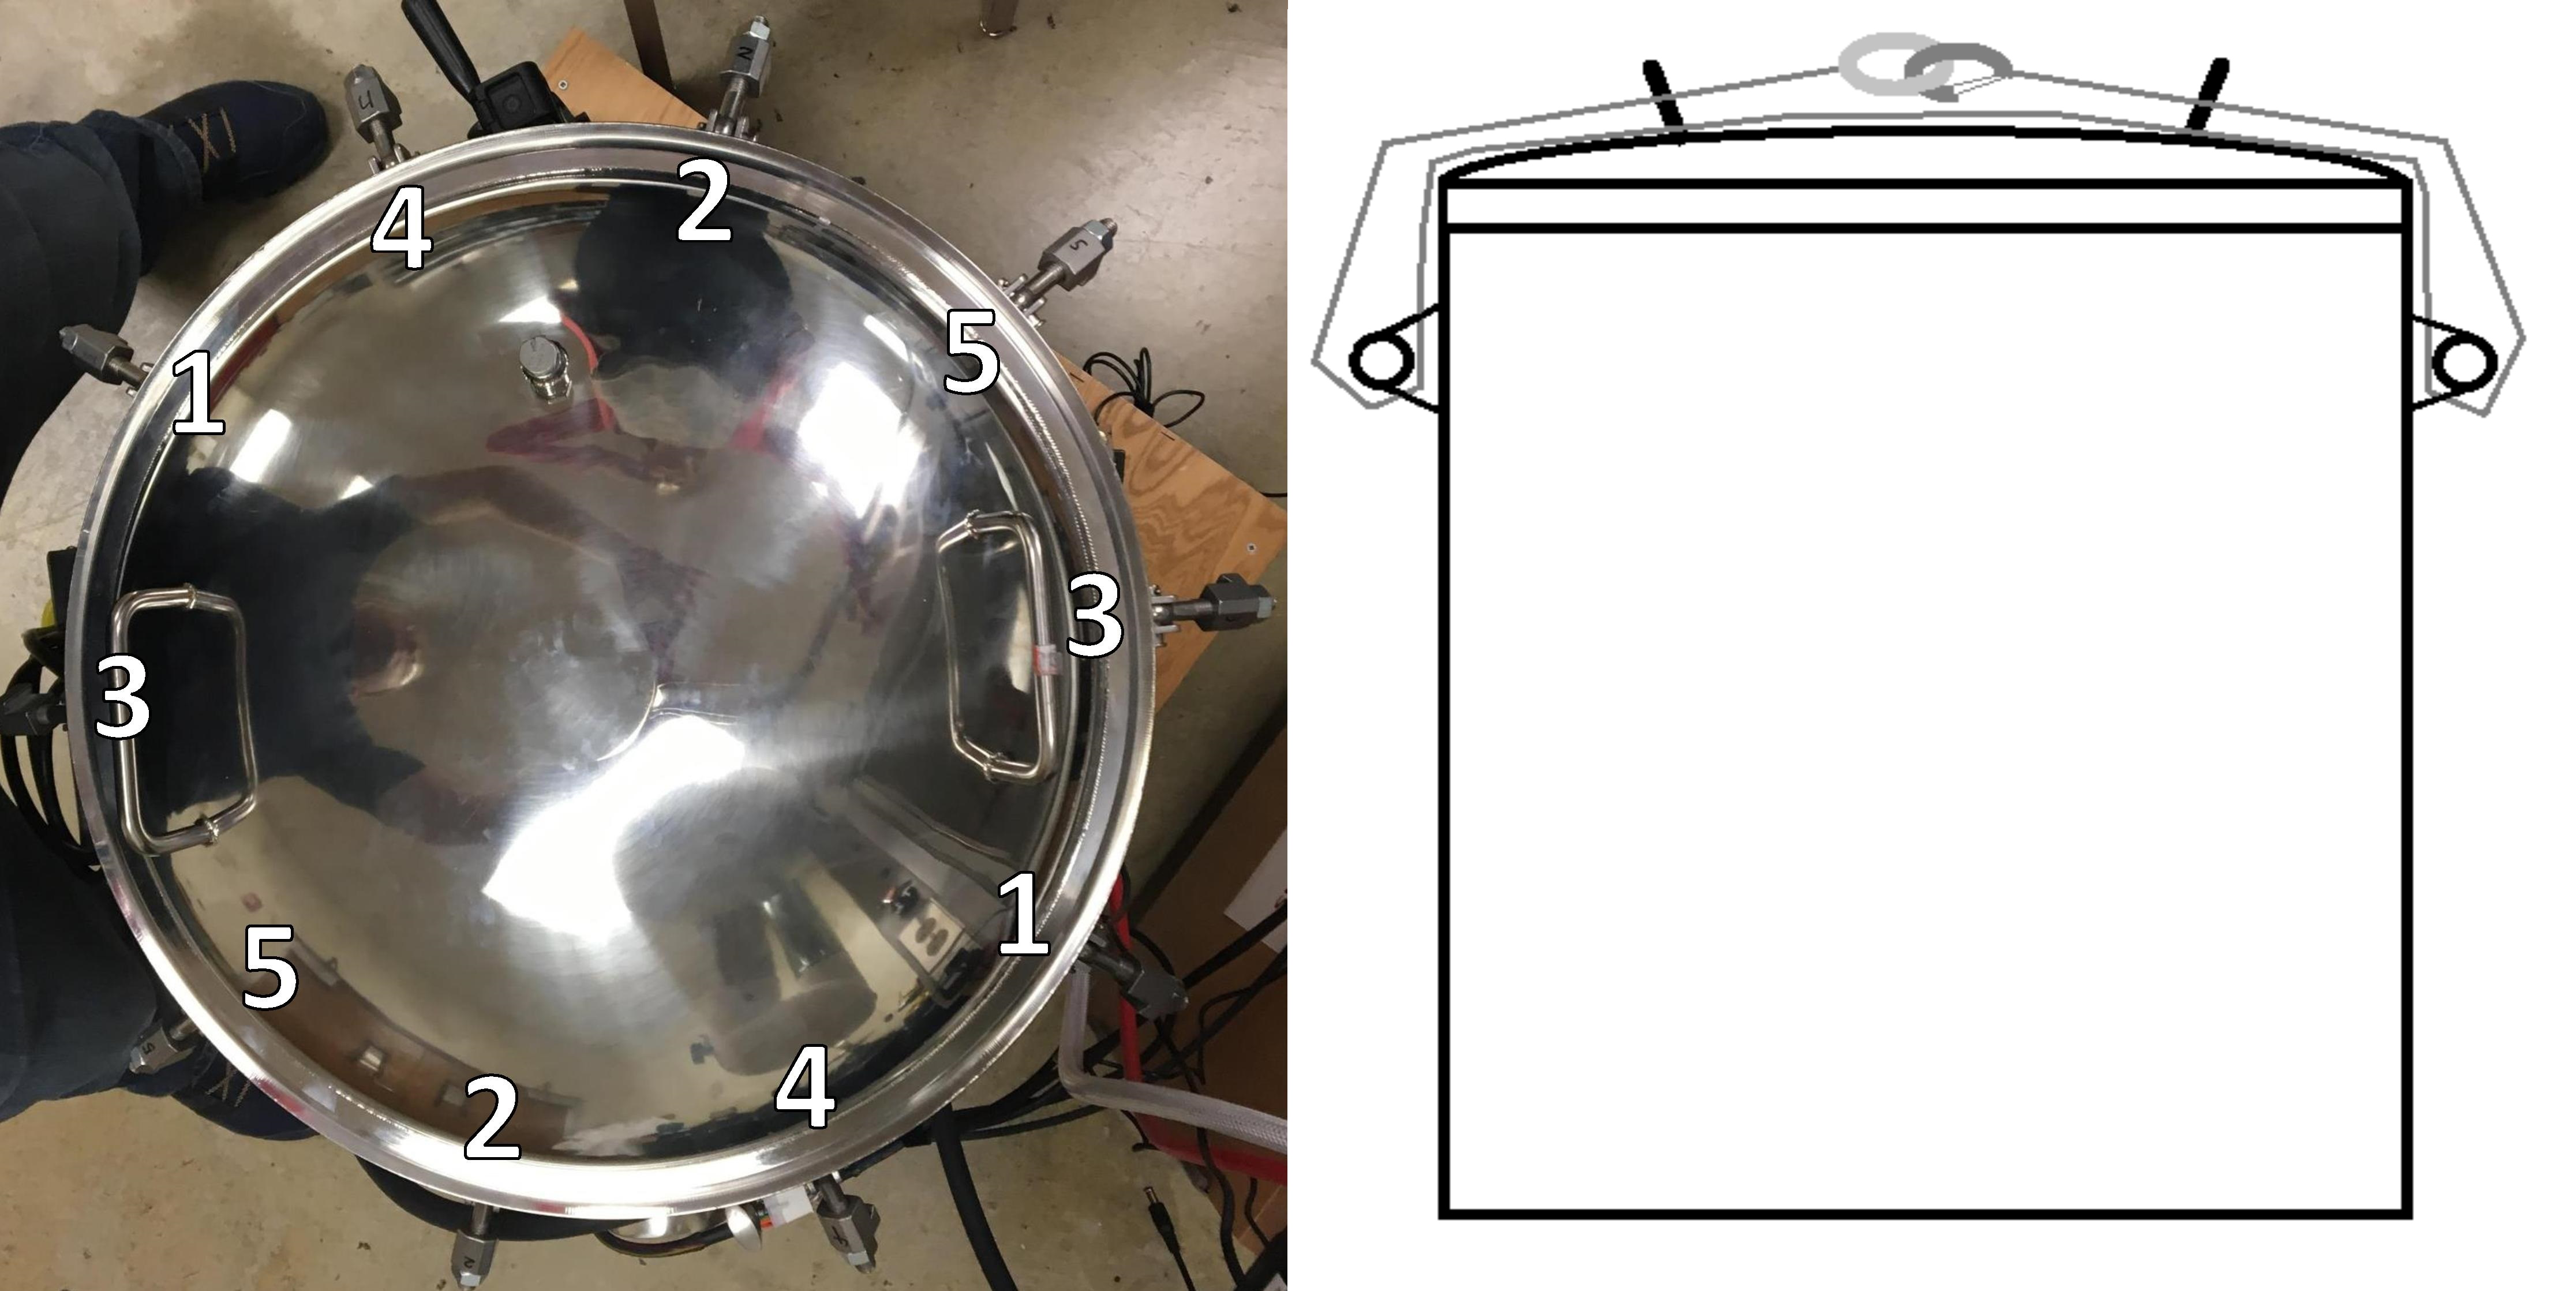
\includegraphics[width=0.5\textwidth]{./PV_lid_secure.jpg}\{\#fig:sec\_lid
  --\textgreater{}
\item
  Pressurize the vessel

  \begin{itemize}
  \tightlist
  \item
    \textbf{Safety glasses are required for everyone in the lab anytime
    the vessel is pressurized}
  \item
    The absolute pressure in the vessel can be read at the bottom of the
    TADA\_UI window and should be plotted on the graph

    \begin{enumerate}
    \def\labelenumii{\arabic{enumii}.}
    \tightlist
    \item
      Ensure the ball valve connecting the regulators to the inlet hose
      is closed (valve handle perpendicular to the flow)
    \item
      Fully open the rotameter on the exhaust of the pressure vessel by
      \textbf{gently} rotating the rotameter knob counterclockwise
    \item
      If it has not been done earlier in the day, slowly open the
      cylinder valve all the way and then turn back one quarter turn
    \item
      Once the regulators are pressurized, ensure the cylinder has
      enough pressure for the next run and the low pressure regulators
      are not over-pressurized (adjust the regulators as needed)
    \item
      Slowly open the ball valve to allow air to flow into the sealed
      pressure vessel
    \item
      Slowly close the rotameter (rotate the knob clockwise) until the
      air flow reads 25 SCFH (The flow rate is read at the middle of the
      floating ball)
    \item
      Allow 1-2 minutes for equilibrium to be reached initially
    \item
      Adjust pressure in vessel using low pressure regulator until the
      absolute pressure reading in the TADA\_UI is highlighted green
      indicating that the pressure in the vessel is sufficiently close
      to 1 atm (760 torr +/- 2 torr)

      \begin{itemize}
      \tightlist
      \item
        This is easier with two people. One to read the pressure off the
        TADA\_UI and the other adjust the regulator
      \item
        While pressurizing, make sure that the rotameter reads about 25
        SCFH. This may take some adjusting back and forth.
      \item
        Allow at least 20 secs for equilibration each time the pressure
        is changed
      \end{itemize}
    \item
      Ensure that there are no leaks around the lid before proceeding

      \begin{itemize}
      \tightlist
      \item
        \textbf{Leak protocol:} If a loud, high pitched noise is heard
        or the pressure read on the TADA\_UI fails to rise, there is
        likely a leak. If this occurs, do the following:

        \begin{enumerate}
        \def\labelenumiii{\arabic{enumiii}.}
        \tightlist
        \item
          Identify where the leak is happening (using the sound or Snoop
          A.K.A. Soapy water)
        \item
          If the leak is happening anywhere besides the O-ring,
          immediately close the ball valve and allow the vessel to fully
          vent to ambient pressure to fix the leak
        \item
          If the leak is happening somewhere along the O- ring, verify
          that there is no debris or wires breaking the seal. If a seal
          break from debris or wires is found, immediately close the
          ball valve and allow the vessel to fully vent to ambient
          pressure to fix the leak
        \item
          If there is no debris or wires breaking the seal, use the
          wrench to slowly tighten the clamp nuts around the leak until
          it stops
        \item
          If none of these steps work or you suspect a different
          problem, immediately close the ball valve and allow the vessel
          to fully vent to ambient pressure to fix the leak
        \end{enumerate}
      \end{itemize}
    \end{enumerate}
  \end{itemize}
\item
  Look through the sight glass on the pressure vessel and ensure the
  vessel is sufficiently dark to see any flame from the mirror on top of
  the furnace
\item
  In the TADA\_UI program, press the ``Choose Target File'' button and
  choose where to save your file

  \begin{itemize}
  \item
    Save all temperature data files in comma separated values (.csv)
    format
  \item
    Example Path:
    \texttt{/home/aitra/Documents/data/compound\_name/filename.csv}
  \item
    File naming convention:

    \begin{itemize}
    \tightlist
    \item
      Filenames will be organized by the following values in order
      separated by underscores (`\texttt{\_}')

      \begin{enumerate}
      \def\labelenumii{\arabic{enumii}.}
      \tightlist
      \item
        Compound name
      \item
        Date of experiment with the format ``YYMMDD''
      \item
        Time of day that data collection began for that run using a 24
        hour clock format ``hhmm''
      \item
        Sample size in microliters (for liquids) or milligrams(for
        solids and gases)
      \item
        Test temperature in degrees Celsius (rounded to the nearest
        integer)
      \end{enumerate}
    \item
      For example: The file name of an AIT experiment where 100
      microliters of hexane were tested at 450 degrees Celsius on March
      19, 2013 at 4:25 pm would
      be:\texttt{hexane\_130319\_1625\_100\_450.csv}
    \end{itemize}
  \item
    This action will reset the TADA for measurement
  \end{itemize}
\item
  Write down everything you know in the TADA window and the lab book
  (i.e.~date, time, sample size, temperatures etc.).
\item
  Begin data collection

  \begin{itemize}
  \tightlist
  \item
    \textbf{Note for unpressurized experiments:} If you are performing
    unpressurized experiments (i.e.~experiments with the lid off) turn
    off the lights and ensure the laboratory is sufficiently dark to see
    any flame from the mirror on top of the furnace \textbf{before}
    beginning data collection.
  \item
    In the TADA\_UI program, press the Enter key or click the ``Collect
    Data'' button on the TADA\_UI
  \item
    The TADA\_UI will keep track of the elapsed time since data
    collection began at the bottom of the window. This may be used to
    time the experiment
  \item
    Press the ``Record'' button on the Camera Suite app to start
    recording
  \end{itemize}
\item
  Press the green or blue button on the ARIA control box that
  corresponds to the physical state of the sample (green for solid, blue
  for liquid) to initiate ARIA sample injection.

  \begin{itemize}
  \tightlist
  \item
    \textbf{NOTICE:} If you need to abort the injection before it
    completes, immediately unplug the AIRA power.
  \item
    If you mistakenly press the wrong button, \textbf{do NOT abort the
    injection}. A button mis-press is inconsequential. Simply allow the
    injection to complete then press the correct button.
  \end{itemize}
\item
  Watch for an ignition event for 10 minutes

  \begin{itemize}
  \tightlist
  \item
    Upon injection, a small temperature drop is always observed. This is
    the start of the 10 minutes
  \item
    A temperature rise above the initial temperature indicates an
    exothermic reaction has occurred
  \item
    An ignition event is defined by the presence of a visible flame
    (visible to either the camera or the operator)
  \item
    An ignition event is characterized by a large, sharp temperature
    rise exceeding \(15 \frac{K}{s}\). This is referred to as a
    temperature spike
  \item
    The experiment ends when one of the following criteria is met:

    \begin{itemize}
    \tightlist
    \item
      An ignition event is observed and the temperature returns to a
      steady state
    \item
      10 minutes pass from the time of injection with no ignition event
      observed
    \end{itemize}
  \item
    Stop and power off the camera with the Capture app about 10 seconds
    after a temperature spike occurs or after a visible flame disappears
  \item
    If temperature spike is observed, allow enough time for the
    temperature to return to a steady state before terminating
    temperature data collection
  \item
    If no ignition event is observed nor expected after a temperature
    rise reaches a maximum, the camera may be stopped before 10 minutes
    have elapsed
  \item
    The TADA may be used to keep track of time. A timer is also provided
    for that purpose.
  \end{itemize}
\item
  If necessary, review the camera footage, looking for a flame
  corresponding to the temperature spike

  \begin{itemize}
  \tightlist
  \item
    This may be done by downloading the footage over the camera WiFi
    using the Camera Suite app
  \end{itemize}
\item
  Record pertinent data and observations in the lab book and the TADA
  \textbf{BEFORE} terminating temperature data collection

  \begin{itemize}
  \tightlist
  \item
    The date of the experiment must be recorded once in the notebook
  \item
    The following data must be present on the same row in the lab
    notebook, in the following order:

    \begin{enumerate}
    \def\labelenumii{\arabic{enumii}.}
    \tightlist
    \item
      Time of day that data collection began
    \item
      Compound name
    \item
      Sample size in microliters (for liquids) or milligrams (for solids
      and gases). Solids will have an exact initial and final mass
      included instead of nominal mass.
    \item
      Set-point temperature of the furnace
    \item
      Test temperature in degrees Celsius (NOT rounded)

      \begin{itemize}
      \tightlist
      \item
        This should be the internal flask temperature (Thermocouple 4)
        prior to injection
      \end{itemize}
    \item
      Indicate the type event that took place (``h'' or ``hot'' for
      hot-flame ignition, ``c'' or ``cold'' for cool-flame ignition and
      ``n'' or ``none'' for no ignition)

      \begin{itemize}
      \tightlist
      \item
        If the flame is bright yellow/orange, this is considered a
        hot-flame autoignition
      \item
        If the flame is faint or blueish, and does not show any yellow,
        orange, or red color, this is considered a cool-flame
        autoignition
      \end{itemize}
    \end{enumerate}
  \item
    If any item is not applicable write down N/A in its place
  \item
    If any item is unknown, leave it blank until it can be determined
  \item
    Optionally, leave any pertinent comments about the experiment next
    to or directly under this row of data (There is a `notes' section in
    the TADA UI window for this purpose)
  \item
    Record the same data in the corresponding fields in the TADA UI
    \textbf{before} terminating temperature data collection
  \item
    The lot number and/or sample number of the compound container with
    the supplier and any other pertinent information related to the
    source of the compound should be recorded at least once in the lab
    notebook when first being used. Ensure that these data are present.
  \item
    Likewise ensure the lot number of the air cylinder being used is
    also recorded when it was first brought into use.
  \end{itemize}
\item
  After the experiment ends, terminate data collection

  \begin{enumerate}
  \def\labelenumii{\arabic{enumii}.}
  \tightlist
  \item
    Press the Enter key again to stop data collection (the red light on
    the TADA should stop blinking)
  \item
    If you haven't already, press ``Recording'' button on the Camera
    Suite app to stop recording
  \item
    Shut down the camera from the Camera Suite app
  \end{enumerate}
\item
  Set furnace to next temperature

  \begin{itemize}
  \tightlist
  \item
    \textbf{Note for unpressurized experiments:} If you are performing
    unpressurized experiments (i.e.~experiments with the lid off) you
    may safely skip the next \textbf{four} steps. Ensure before
    proceeding that the vessel is being vented by the snorkel.
  \end{itemize}
\item
  Wait about 20 minutes after ignition to allow for the pressure vessel
  to be purged of the combustion products. If there was no ignition,
  only wait 10 minutes for the pressure vessel to purge after the
  experiment ends
\item
  After the purge time has ended, depressurize the vessel

  \begin{enumerate}
  \def\labelenumii{\arabic{enumii}.}
  \tightlist
  \item
    Turn off the inlet air flow using the ball valve
  \item
    Fully open the rotameter by gently turning the knob counterclockwise
  \item
    Wait until the pressure vessel is \textbf{fully} depressurized
    (i.e.~the rotameter reads zero)
  \end{enumerate}
\item
  Remove the pressure vessel lid by \textbf{first} loosening and
  disengaging the clamps and \textbf{secondly} removing the safety cable

  \begin{enumerate}
  \def\labelenumii{\arabic{enumii}.}
  \tightlist
  \item
    Loosen the clamps using a 3/4" wrench
  \item
    Break the seal on the lid by briefly lifting the lid with the safety
    cable still in place
  \item
    Remove the safety cable from the vessel
  \end{enumerate}
\item
  \textbf{Simultaneously} lift off the lid and place snorkel inside the
  pressure vessel between 6" and 10" over the furnace (this may be done
  with 1 person)

  \begin{enumerate}
  \def\labelenumii{\arabic{enumii}.}
  \tightlist
  \item
    Lift the hood sash to allow the lid to be placed back inside
  \item
    Pull the bell of the snorkel up to allow the snorkel to swing up
    once the lid is removed
  \item
    Swing the snorkel to a position above the vessel
  \item
    Pull the bell back down to the end of the snorkel and let it fall on
    top of the lid so the snorkel will fall into place once the lid is
    removed
  \item
    Ensure the snorkel is loose enough to fall down into the vessel upon
    removing the lid
  \item
    Remove the lid by pulling directly upward before moving laterally
    and allow the snorkel to fall down into the venting position inside
    the vessel
  \item
    Place the lid carefully back in the hood and close the sash, running
    the lid outlet hose through the small opening in the corner of the
    sash
  \item
    Ensure the snorkel is placed properly and is venting the vessel
  \end{enumerate}
\item
  Remove the camera from the vessel

  \begin{itemize}
  \tightlist
  \item
    Connect it to the computer to begin video extraction if you haven't
    done that already
  \item
    Connect the camera to power to charge if necessary
  \end{itemize}
\item
  Remove any syringe or weigh boats used in the previous experiment

  \begin{itemize}
  \tightlist
  \item
    \textbf{Use gloves when doing this}
  \item
    For experiments with solid compounds:

    \begin{enumerate}
    \def\labelenumii{\arabic{enumii}.}
    \tightlist
    \item
      Carefully remove the funnel and the weigh boat avoiding losing any
      residue from both of them
    \item
      Using a \textbf{clean} chemical spatula, carefully scrape any
      compound residue from the funnel into the weigh boat, cleaning the
      funnel of as much residue as possible
    \item
      Place the weigh boat on the scale you tared earlier

      \begin{itemize}
      \tightlist
      \item
        The mass displayed should be negative, this is the approximate
        mass that actually entered the flask multiplied by \(-1\)
      \end{itemize}
    \item
      Note this weight as the final sample size in the lab notebook
    \item
      Rinse out the funnel of any remaining residue with acetone
    \item
      Dispose of any weigh boats in the solid waste
    \end{enumerate}
  \end{itemize}
\item
  Clean out the flask between measurements by blowing hot air into the
  flask for 5 minutes using the heat gun on the low setting

  \begin{itemize}
  \tightlist
  \item
    The heat gun should \textbf{only} be plugged in to the outlet when
    in use
  \item
    Do not point the heat gun towards the ARIA at any time
  \end{itemize}
\item
  Extract, save and appropriately rename the video data between
  experiments (See Section refsec:vid\_ex). Remember to delete the video
  off the camera once you have made sure that it is saved to the
  computer.
\item
  Once the next temperature is reached, allow the system to come to
  equilibrium

  \begin{itemize}
  \tightlist
  \item
    The ``Temp Ready'' indicator in the TADA\_UI window should turn
    green when the system has come to an acceptable equilibrated state
  \end{itemize}
\item
  Once the system is at equilibrium, start this procedure over from step
  1 (Measure Out Sample)
\end{enumerate}

\hypertarget{shutdown}{%
\subsection{Shutdown}\label{shutdown}}

The following should be done before leaving the lab at the end of every
work day or any time the setup is not in use:

\begin{enumerate}
\def\labelenumi{\arabic{enumi}.}
\tightlist
\item
  Power off the furnace
\item
  Shutdown TADA

  \begin{enumerate}
  \def\labelenumii{\arabic{enumii}.}
  \tightlist
  \item
    Close the TADA\_UI program
  \item
    Unplug TADA's USB connection
  \item
    Unplug the wall power from the TADA power supply
  \end{enumerate}
\item
  Shutdown ARIA and store accessories

  \begin{enumerate}
  \def\labelenumii{\arabic{enumii}.}
  \tightlist
  \item
    Unplug the ARIA power supply cable
  \item
    Remove and store any ARIA accessories used that day (leave the ring
    stand in place)
  \item
    Clean the funnel with appropriate solvents and dispose of the waste
  \item
    Appropriately, discard the contents of beakers and prepare them for
    dish washing
  \item
    Discard any residual sample in syringes and store them in the
    syringe box in the AIT drawer without rinsing
  \item
    Store all chemicals in the appropriate cabinets
  \end{enumerate}
\item
  Remove any organic solid residue from working surfaces (See Section
  refsec:spill\_solid)
\item
  Ensure all air systems are depressurized

  \begin{enumerate}
  \def\labelenumii{\arabic{enumii}.}
  \tightlist
  \item
    Ensure the ball valve is closed (the handle should be perpendicular
    to the flow)
  \item
    Slowly close the cylinder valve all the way
  \item
    Open the ball valve by turning the handle parallel to the flow
  \item
    Wait until both regulators depressurize
  \item
    \textbf{Leave the ball valve open}
  \end{enumerate}
\item
  Extract all data to the computer and appropriately rename them (Refer
  to Section refsec:data)
\item
  Determine if the flask should be changed, if so write this down in the
  lab notebook
\item
  Turn the camera Wi-Fi off then shut down and unplug the camera
\item
  Close all programs and shut down the computer
\end{enumerate}

\begin{itemize}
\tightlist
\item
  A hot furnace may be left with the pressure vessel open and the
  snorkel venting it without waiting for it to cool
\item
  Under normal use, disposable gloves may be thrown into the normal
  trash receptacle instead of solid chemical waste
\end{itemize}
